\documentclass[conference, letterpaper]{sig-alternate-05-2015}

\usepackage{graphicx,balance,comment,times,amsmath,slashbox,url,multirow,algorithmic,color,amssymb,verbatim,float,chngcntr,enumitem}
\counterwithin{paragraph}{subsection} % makes paragraph depend on chapter
\usepackage{algorithm2e}
\usepackage{epstopdf}
\newcommand{\rednote}[1]{\color{red}{ \em #1 }\color{black}}
\newcommand{\recheck}[1]{\color{blue}{ \em #1 }\color{black}}
\newcommand{\blue}[1]{\color{blue}{ \em #1 }\color{black}}
%To hide notes: uncomment the following line
%\renewcommand{\rednote}[1]{}
%\renewcommand{\recheck}[1]{}

\usepackage{caption}
\usepackage{subcaption}
\def\unit#1#2{\hbox{#1$\,\textrm{#2}$}}
\newtheorem{theorem}{Theorem}[section]
\newtheorem{lemma}[theorem]{Lemma}
\newtheorem{proposition}[theorem]{Proposition}
\newtheorem{corollary}[theorem]{Corollary}

\newenvironment{definition}[1][Definition]{\begin{trivlist}
\item[\hskip \labelsep {\bfseries #1}]}{\end{trivlist}}

\newcommand{\trajSummary}{TrajSummary\ }
\newcommand{\thresh}{THRESH\ }
\newcommand{\modal}{MODE-EST\ }
\newcommand{\lthAware}{L-AWARE\ }
\newcommand{\weightLP}{\operatorname{WCD}}
\newcommand{\LP}{L^2}
\newcommand{\UN}{L^\infty}
\newcommand{\od}{\operatorname{OD}}
%\newcommand{\roadSegDist}{\operatorname{roadSegDist}}
\newcommand{\rawlat} {\operatorname{rlat}}
\newcommand{\rawlon} {\operatorname{rlon}}
\newcommand{\rawtime} {\operatorname{rtime}}
\newcommand{\lat} {\operatorname{lat}}
\newcommand{\lon} {\operatorname{lon}}
\newcommand{\timev} {\operatorname{time}}
\newcommand{\maxlat} {\max_{\lat}}
\newcommand{\minlat} {\min_{\lat}}
\newcommand{\norm}[1]{\left\lVert#1\right\rVert}
\newcommand{\summClus} {S}
\newcommand{\setSummClus} {\mathbf{S}}
\newcommand{\meanTraj} {\bar{t}}

\begin{document}
\title{MoSum: Spatio-temporal Mobility Summary of Individuals}
\maketitle
\begin{abstract}
Mobility data of people is being increasingly recorded by location sensing applications such as GPS traces and Cellular Network Records. Such large-scale location data of people is capable of providing rich mobility context information about how, where and when an individual moves. These insights are useful in several domains such as hyper-targeted advertising, city transportation planning and cellular network planning. While mobility data is capable of providing such interesting information, techniques to summarize a spatio-temporal mobility of a individual is non-existent. We aim at coming up with a framework to do the same.We also propose a novel way to store mobility signatures of a person, which in turn provides a powerful mechanism for solving various use-cases that can rely on regular movement pattern of an individual (such as next-location prediction and anomalous movement detection).
\end{abstract}
\section{Introduction}
%% 1. Location data is being increasingly collected and is useful. (has the potential to unlock several novel usecases such as city transportation planning and user interest analysis)
Advances in GPS-based applications and ubiquitous connectivity have enabled collection of vast amounts of location data describing the movement of humans and animals. Currently, location traces of millions of people are being collected by various applications. In addition, location traces of a vast majority of the population are inherently collected by cellular network operators in the form of \emph{Call Detail Records}, which continuously log the base-station to which the user is connected. This large-scale location traces of people enables understanding the movement pattern of objects, and opens a plethora of location-enabled applications such as location prediction, mobility-intent identification and anomaly detection. 

%% 2. Human mobility data opens new avenues
Location data can be used to analyze user interactions in the physical space. Insights from location data enable determining user interests, demographics and who they hangout with based on where, how and when people go to different locations such as stadiums and malls. Hence, location data -- similar to social networking data --enables enterprises to create new revenue streams. A primary challenge in enabling new applications is inferring insightful movement patterns from the raw location traces. Existing studies have focused on identifying hangouts of an individual, such as home/work and other frequently visited places. Hangouts provide a spatio-temporal signature of the person in terms of where the person hangs out. However, such algorithms do not indicate the mobility pattern of the user. 

%%Such surveys are inherently limited by the number of people surveyed, and in the type of responses elicited by the users; most often they collect the home/office locations and time-of-travel from around 1\% of the population, and prepare an Origin-Destination (OD) matrix that shows how many users might move from one part of the city to another. Such data is used to plan bus and trains in the city. Contrast planning the city transportation with location data. Information of precise user movements every day from Telcos or other popular location tracking applications like Waze~\cite{waze}, will provide them the actual OD matrix based on real-movement data, and not from the subjective responses from the users. In addition, the fine-grained data with advanced analytics will also help them understand who, when, why, where and how the users move at a fine-granular level. This helps the smarter city transportation departments to precisely plan multi-modal transportation systems. 
%%Location data also opens opportunities to create additional revenue streams. Popular social networking enterprises now mainly generate revenue by utilizing user interactions in the virtual space (using social-network posts and search queries) for personalized advertizing -- without breaching user privacy. Similarly, location data has the potential to utilize how users move in the physical world and monetize the data by providing them smart hyper-targetted advertizements. For example, a user who often visits a coffee-shops is the ideal candidate to send promotions to a new coffee shop that has opened on the commute path between the user's home and office. Many such queries can be enabled on location data to solve interesting usecases. 

%% 3. The time-series of location traces can be used to infer home,work, etc. Such summaries are useful for many applications on infering where the user hangs out. People want to construct summaries like hangouts etc. How do we do this for mobility pattern detection?


%% Why mobility summary
%% In this industry, regular traj query is most ofnte used. Pepple go back to raw trajs to compute -- evertime. We need better representation.
\subsection{Motivation}
Mobility summary of an individual succinctly describes frequent paths taken by the user. Mobility summary is the natural abstraction for many higher level applications that utilize ``frequent-mobility based queries'', where an application can query frequent movement patterns -- instead of all the trajectories of the user -- to infer some insight.
Examples of frequent-mobility based queries include: (1) users who frequently pass through a given place such as a coffee shop, (2) Next-path prediction problem where user's future path is predicted based on current path and a history of user trajectories, and  (3) Anomalous Trajectory Detection where outlier trajectories of a user need to be filtered. Such queries are efficiently solved by a one-time computation of mobility summary. Applications can then query the summary to provide insights. Hence, mobility summary enables efficient and fast-lookup for many movement-based queries that rely on computing frequent trajectories of an individual. Mobility summary extraction involves working with trajectories. A \textbf{trajectory} can be defined as a series of points in the spatial domain , spread over a certain time period.

%For example, summary mobility enables identifying users who regularly pass through a coffee shop or digital billboards, so that advertisements can be targeted to the most appropriate and regular users. Mobility summary provides a novel and efficient way to solve well-known trajectory queries. Solutions to next-location prediction and anomalous movement detection are reduced to a simple lookup operations on few representative summary trajectories -- rather than repeatedly sifting through thousands of trajectories of a user using a complicated model. 
%% What is done till now
% Our contribution
The primary objective is to construct the mobility summary for individual users considering the spatial aspect. A system needs to be built  which takes as input, a time-series of user's location traces and outputs a set of weighted representative summary trajectories of the user, which describe the user's mobility pattern. 
\subsection{Objectives}
%We score each summary trajectory proportional to how often the user has traveled along that path. The output of \trajSummary is a compact representation of user's mobility pattern. 
The broad objectives of the work are as follows:
\begin{itemize}
\item{\textbf{Trajectory Preprocessing:}}
This involves cleansing of the raw data and methods to extract meaningful trips or trajectories out of an input chunk, which is a collection of three tuples \emph{$\langle$ latitude, longitude, timestamp $\rangle$ }
\item{\textbf{Trajectory Similarity Analysis:}}
Attempts to define a similarity measure between two trajectories is the foundation of any kind of aggregation, or clustering. The existing measures are discussed, and a new scheme or definition for similarity between trajectories has been proposed. The proposed similarity measure is designed considering human mobility.
\item{\textbf{Trajectory Clustering:}}
This involves development of a trajectory clustering scheme. Given an input of trajectories, and a method which defines a similarity between two trajectories, the goal is to devise a clustering algorithm which outputs the final grouping of trajectories such that the final clusters define the mobility summary.
\item{\textbf{Trajectory Summarization:}}
Once the clusters are formed, a representative trajectory for each of the cluster needs to be computed and that would form the entire trajectory summarization. A method for storing the trip summaries of a person in a hierarchical fashion using this summarization will also be developed. 
\item{\textbf{Applications of Mobility Summary:}}
Following applications of \emph{mobility summary} will be attempted-Next Path Prediction, and Anomaly Detection.
\end{itemize}



\section{System Overview}
\label{sec:system}
\begin{figure}
\centering
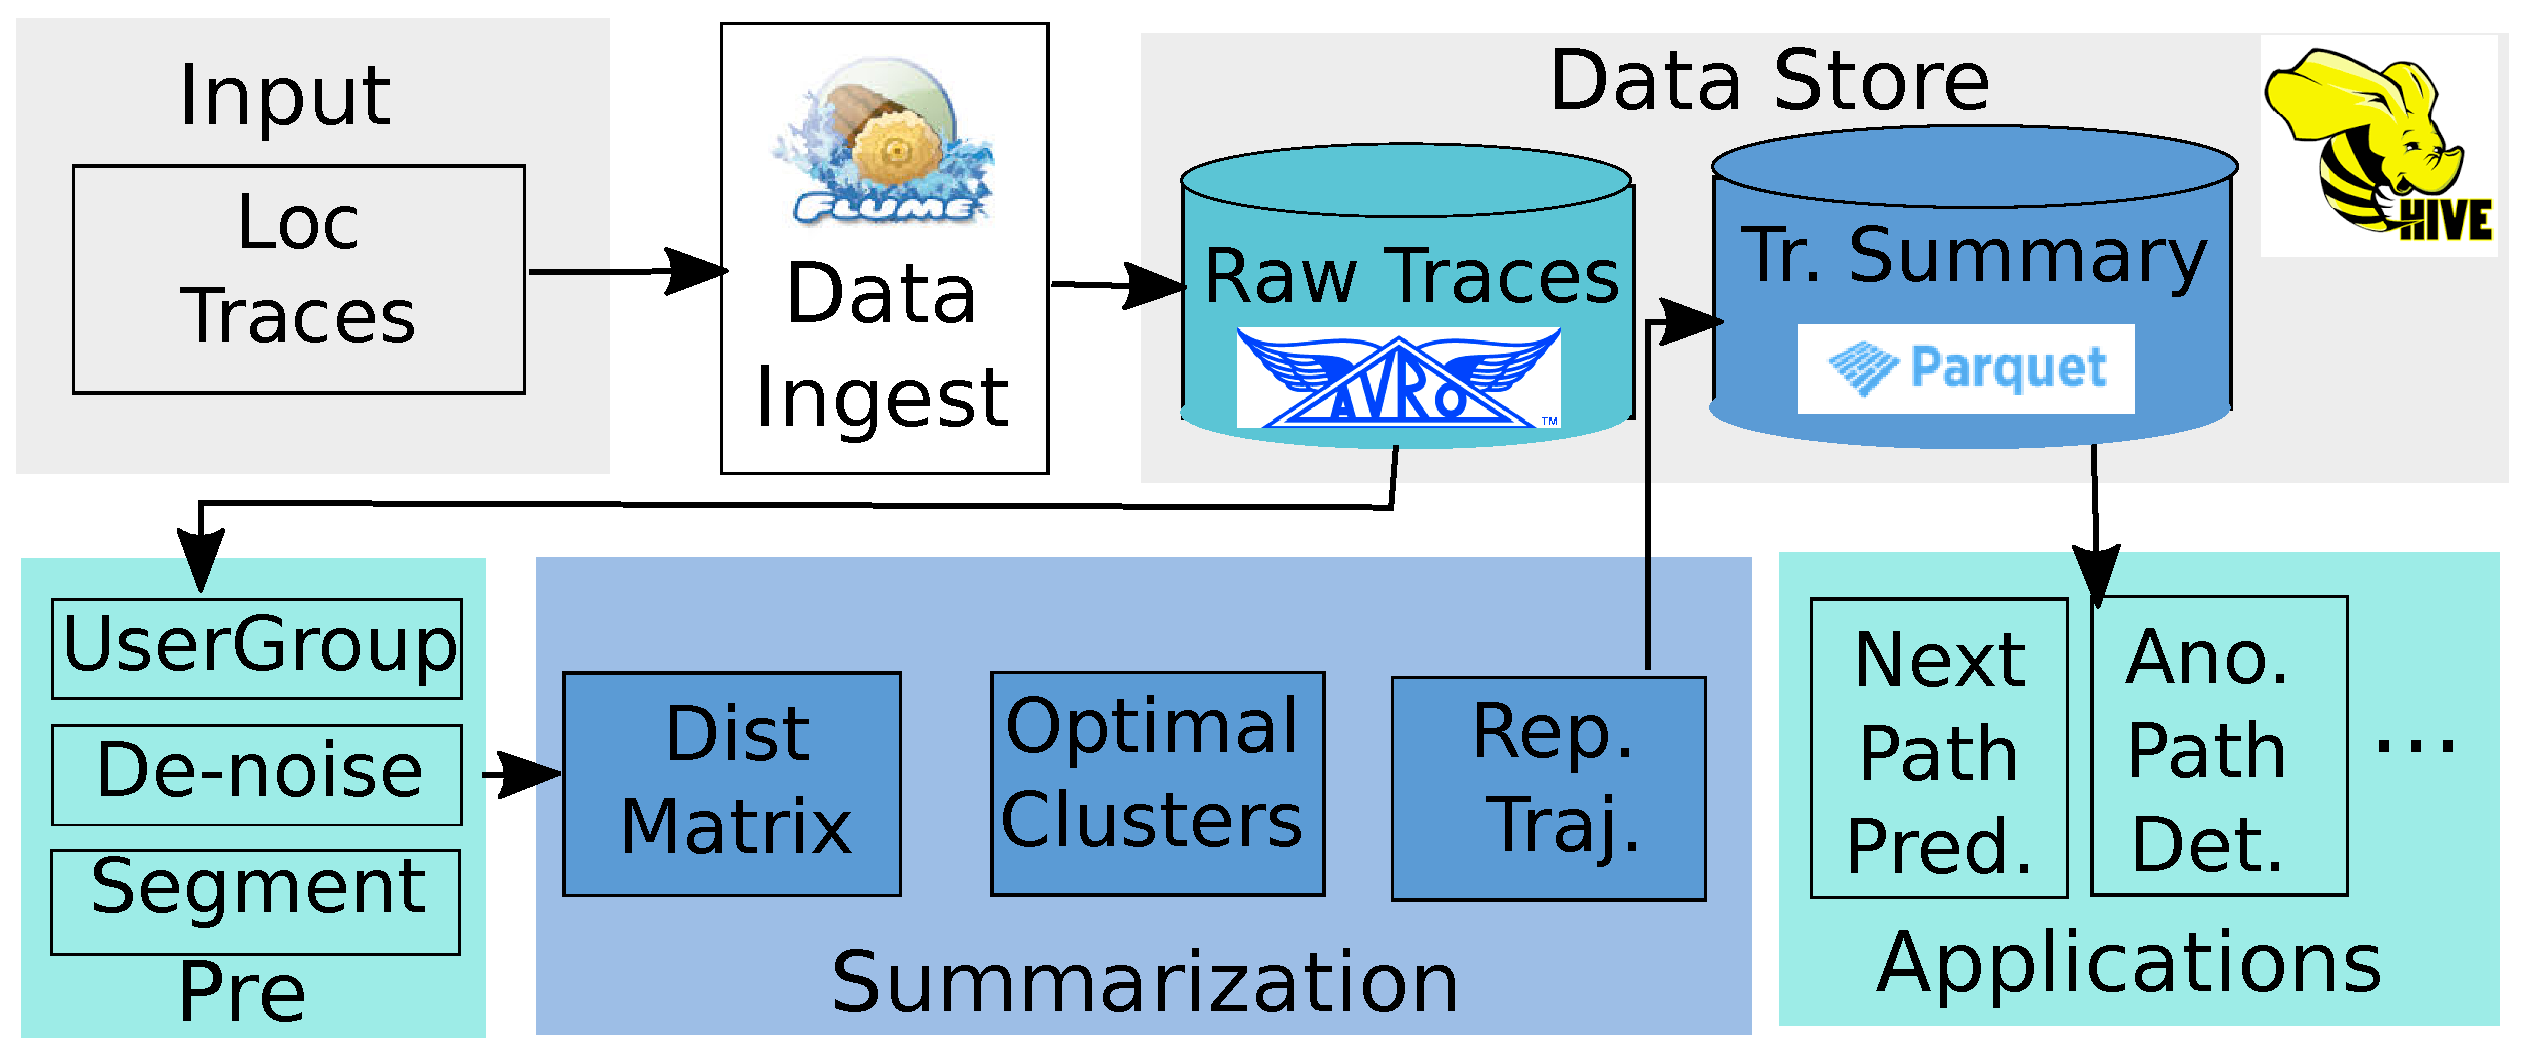
\includegraphics[scale=0.15]{figs/arch1.eps}
\caption{Conceptual Architecture}
\label{fig:flow}
\end{figure}

\begin{figure*}
    \centering   
		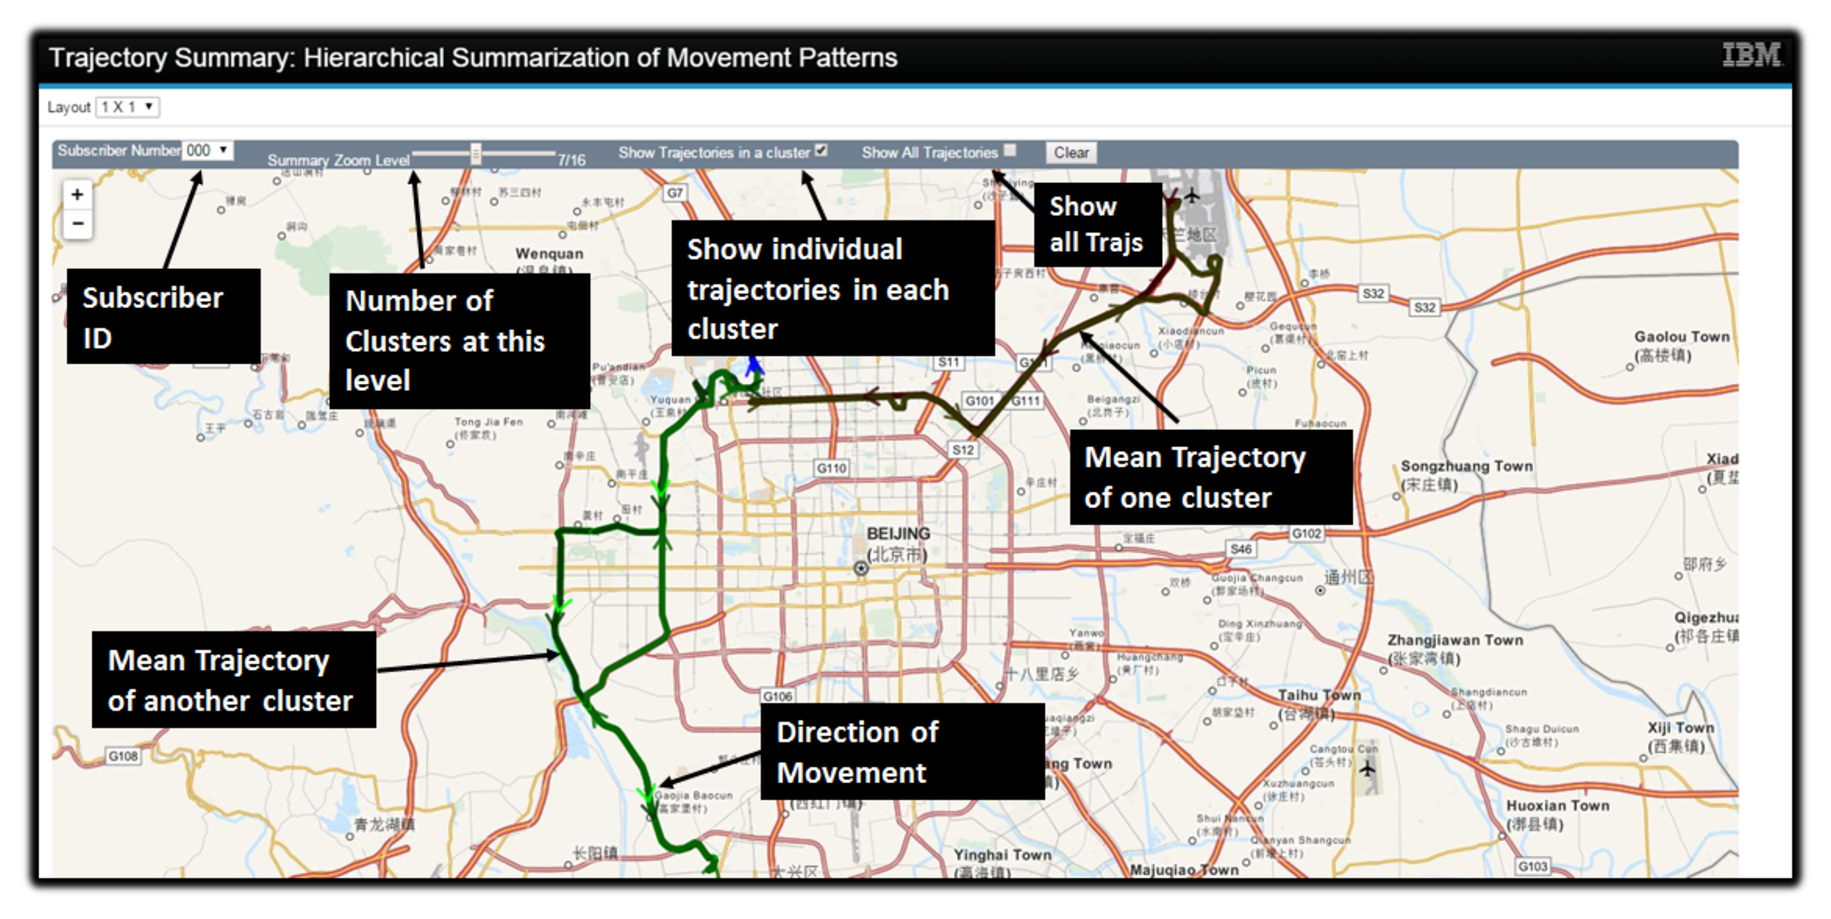
\includegraphics[scale=0.5]{figs/visual.eps}
		\caption{Visualization Framework.}
		\label{fig:vis}  
\end{figure*}

We have developed \trajSummary on Hadoop-based framework for processing large-scale movement summaries. Fig \ref{fig:flow} describes the conceptual architecture. 

\paragraph{Data Ingestion} 
The input to the system is a continuous stream of raw location traces of different users. Each location trace record at-least consists of user identifier, spatial coordinates (latitude and longitude) and time of sample. We use Apache Flume~\cite{flume} to load the real-time traces being continuously deposited in a pre-configured landing directory. The Flume sink then writes the records on the HDFS file system in AVRO format. This data will be mapped as an external table, which is accessible to our analytics modules implemented in Apache Hive~\cite{hive}. Note that the data ingestion happens in real-time; Flume converts and stores the AVRO location samples as and when the location samples arrive in our landing directory

\paragraph{Pre-processing}
\label{sec:preprocess}
Pre-processing stage and the later steps are currently implemented as Batch Analytics. Batch Analytics is executed periodically, which aggregates the records in the past period, and creates data that can be used by the analytics.

In the pre-processing stage, we perform three main tasks: User Grouping, De-noising and Trajectory Segmentation. User Grouping groups location samples of all users into a Hive table in Parquet format. Parquet format is adopted since it provides columnar compression which is useful for our data-sets. This step is necessary since the data is flowing into the system from multiple users at the same time, and our analytics input is the location traces (trajectories) of individual users.

De-noising module filters the outlier GPS traces. We use existing outlier detection algorithms to prune the raw locations~\cite{Yuan2013,Zheng2009}. Such techniques estimate the speed between the consecutive sample points of a user, and prune the points if the speed is greater than a certain threshold (\unit{300}{kmph} in our case).

Trajectory Segmentation identifies the meaningful trips of a user from raw location traces. It utilizes well-known stay-point estimation approaches~\cite{trajcut3}, and stores the \textit{User Trajectories} table. Each trip is stored as an ordered set of 3-tuples $\langle \operatorname{latitude},\operatorname{longitude}, \operatorname{time} \rangle$.

\paragraph{Summarization}
Summarization module is the main contribution of the paper. It inputs the data from the \textit{User Trajectories} table, and stores the user-summaries into the \textit{Traj. Summary} table. We propose and evaluate techniques to compute the summaries for a set of user-trajectories. We show that optimal movement summaries requires understanding of three fundamental concepts: (1) Defining the distance metric between two user trips (Section~\ref{sec:trajDist}); (2) Finding the optimal cluster of user trips that represents a trajectory summary (Section~\ref{sec:trajCluster}); and (3) Representing summaries using a representative trajectories, which can be utilized by the downstream applications (Section~\ref{sec:repTraj}). 

\paragraph{Applications}
The summarization module provides a compact abstraction for applications that query ``frequent-mobility''. Several use-cases can utilize the summary representation of the mobility pattern to provide insights. Next-path prediction problem and Anomalous Movement Detection are example applications that benefit from \trajSummary.

\paragraph{Visualization}
\label{sec:vis}
Fig. \ref{fig:vis} shows a screen-shot of the visualization framework which has been created to work with the trajectories, and the summaries of the user. The interactive framework shows the mobility summary different users. The tool allows exploration of clusters formed at various zoom levels of space. With this flexibility, the tool allows choosing arbitrary level of abstraction of movement summary (e.g., at a city level or at a more granular trajectory level). 
%Once the number of clusters( say k) is set, the k clusters formed will be shown, each cluster in a different colour. 
The tool shows the representative trajectory of each cluster; the thickness is proportional to the number of trajectories in the cluster. Further, each cluster can be individually chosen and inspected. 

\begin{comment}
Various trajectory similarity metrics, which give an estimate of the trajectory distance, have been proposed. Standard LP-Norm and ERP have been shown to be metrics~\cite{Chen2004}, where as other heuristic functions (such as LCSS, DTW, EDR) are non-metrics~\cite{Vlachos2002,Yi1998,Chen2005}. We enhance LP-Norm to construct ``Weighted LP-Norm"', where more weights are given to the points closer to the origin and destination. This is based on the observation that, generally, a user's meaningful trip has an associated intention of commuting between two end-points (such as commuting to work or grocery shop visit).

\noindent\textbf{3. Trajectory Clustering}: 
In this module, hierarchical clustering is applied on the previously computed distance matrix. We choose hierarchical clustering because it gives us a way to store the trajectories of the user at various levels of granularity. Hierarchical clustering involves the computation of a dendrogram which describes how the trajectories are clustered throughout the various levels. We devise a function to cut the dendogram to form the right clusters based on earth-distance between the trajectory points of a cluster.
%The major obstacle is in finding the right number of clusters('k'). The most widely used method in literature to find the value of 'k' is to draw the plot of the number of clusters vs. Sum of Squared Errors within clusters, and finding the elbow point in the plot. However, in the case of human mobility, the clusters formed at the elbow point are very noisy. The heuristic we apply to come up with tighter, meaningful clusters is to go down the dendrogram, starting from the elbow point and reporting final clusters as and when the maximum point-wise earth-distance between all two trajectory pairs is less than a specified threshold $\delta$.

\noindent\textbf{4. Representative Trajectory:} 
We summarize the significant clusters by a representative trajectory for that cluster. We utilize the median trajectories~\cite{median1} because it provides parts of actual user traveled paths as representative trajectory.\\
\end{comment}
\section{Formulation and Overall flow}
\begin{figure}[!htb]
\centering
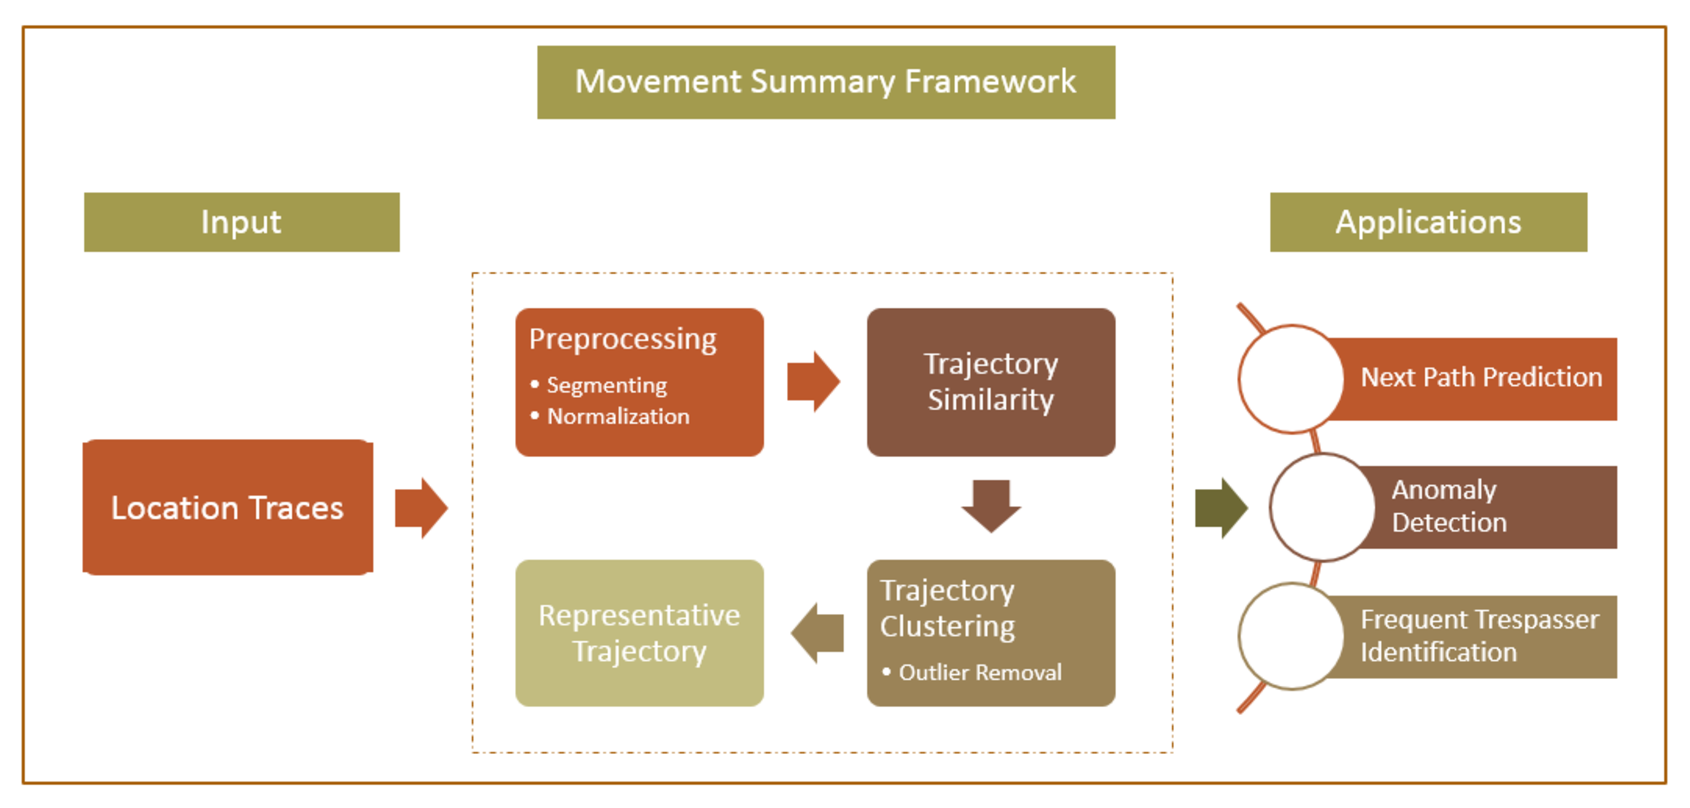
\includegraphics[scale=0.6]{figs/overallflow.eps}
\caption{Overall Flow}
\label{fig:components}
\end{figure}

Figure \ref{fig:components} provides the different components for computing the Mobility Summary, which in turn can be used a variety of applications that rely on frequent-mobility based queries.The various components of the flow are described briefly below: 

%% 1 Trajectory Segmentation
%% 2. Trajectory Similarity
%% 3. Clustering
%% 
\paragraph{Input}
The input in the form of a raw collection of three tuples, which are the location traces of the person or user.
\paragraph{Preprocessing}
Pre-processing consists of the steps segmenting which is the process of making meaningful trips out of the raw traces. The second component is normalization.
\paragraph{Trajectory Similarity} 
This is the module which defines and computes the similarity between all the pairs of trajectories in the dataset. This is a very crucial step as the clustering depends on the goodness of the similarity measure.
\paragraph{Trajectory Clustering}
This module takes as input the similarity matrix formed in the earlier step, and runs a clustering algorithm on it and outputs a final cluster of trajectories. This step also encompasses outlier or anomaly detection.
\paragraph{Representative Trajectory} 
Once we have all the final clusters, we have to come up with on trajectory per cluster which can act as the representative trajectory for that cluster. This task is taken up in this section.
\paragraph{Applications}
The applications of Movement Summary include next path prediction and anomaly detection.
 

\section{Trajectory Clustering}
\label{sec:trajCluster}

A similar problem to \trajSummary is clustering of generic trajectories, which has been studied for different purposes~\cite{Lee2007,Li2010}. We briefly describe and illustrate existing trajectory clustering mechanisms, and show that they do not provide good spatial summaries for trips of individuals. We then propose parametric and non-parametric techniques that utilize different distance metrics for effective clustering of user trips.

\subsection{Trajectory-distance Unaware Techniques}

\paragraph{TRACLUS}
TRACLUS is a frequently used algorithm for clustering trajectories. It is based on the \emph{partition-and-group} framework. TRACLUS relies on discovering similar  sub-trajectories, and doesn't look at them as a whole. In the first phase, the trajectories are partitioned into line segments based on Minimum Description Length principle. Once the trajectories are partitioned, it runs a density based clustering on the line segments based on two parameters, $\operatorname{minPts}$ and $\epsilon$. 
\\
We implemented TRACLUS, and used simulated annealing to arrive at the values of the parameters. TRACLUS was designed to detect animal movement, and trace hurricane patterns. In such cases, sub trajectory similarity played an important rule, which TRACLUS exploits. But in the case of human mobility or movement summarization, we want to look at entire end to end trips, and not delve into the sub-trajectory level. 

\begin{figure}
\begin{center}
\includegraphics[width=3.5cm]{figs/TrajClus_cluster.jpg}
\end{center}
\caption{TRA-CLUS illustration: The large number of trajectories in a large area (in yellow color) are reported as primary cluster}
\label{fig:TrajClus_cluster}
\end{figure}

\paragraph{Swarm}
SWARM is a clustering method which clubs similarly moving objects together in a cluster. If a minimum $m_{0}$ number of individuals in a group fall in the same cluster for at-least a minimum number($min_{t}$) of non-consecutive timestamps, a swarm is reported. A swarm is a closed swarm if neither its Object set nor its Timestamp set can be further extended. The algorithms finds such closed swarms by doing a DFS on all the subsets of object timestamp pairs, with different rules to prune the search space.
To suit our problem, we considered the ordering of the points in the trajectory to be the timestamp value for that point. \\
To suit our problem, we considered the ordering of the points in the trajectory to be the timestamp value for that point. Making this assumption we took all the trajectories of the user to be the set of objects and identified closed swarms. As the points might not be sampled in a similar fashion, SWARM might miss out on similar clusters even though they are close to each other. 

\subsection{Trajectory-distance Aware Techniques}
\label{sec:trajDistClustAlgos}
Standard clustering approaches can be used with the trajectory distance measures mentioned in Section~\ref{sec:trajDist}. However, obtaining optimal clusters that describe meaningful user trip summaries require extensive analysis and experimentation of clustering approaches. We now describe the clustering algorithms and techniques to compute optimal user trip clusters.

\paragraph{DBSCAN}
\label{sec:dbscan}
Density-based spatial clustering of applications with noise (DBSCAN) is a widely used clustering algorithm which clusters closely connected points (dense neighborhoods)~\cite{ref:dbscan}. DBSCAN inputs two parameters: minimum number of neighborhood points ($\operatorname{minPts}$) and a neighborhood distance radius ($\epsilon$). 

Using the above parameters, DBSCAN categorizes each point as a core, reachable or outlier points. A core point is defined as a point which has at-least $\operatorname{minPts}$ within a radius of $\epsilon$. Reachable points are points which has less than $\operatorname{minPts}$ in its $\epsilon$-neighborhood, but there is at-least one core point within its $\epsilon$ distance. Rest of the points are termed as outliers. DBSCAN hence forms a cluster of core points with possible reachable points in the boundary. 

In our application, we show that DBSCAN is not the right clustering method irrespective of the distance metric used because of the fixed selection of neighborhood thresholds ($\operatorname{minPts}$ and $\epsilon$). This hinders the ability to find meaningful summaries in scenarios where users have, say, a mix of long and short trips. Here, we require the long distance trips to have a larger $\epsilon$ than for the shorter trips since such a property allows larger detours for long trips than for short trips. Note that parameter tuning will not yield meaningful summaries in the above cases since: (1) Increasing $\epsilon$ (or decreasing $\operatorname{minPts}$) will lead to clustering a large number of dissimilar smaller trips (small $\operatorname{minPts}$ or large $\epsilon$); or (2) Small values of $\epsilon$ may unnecessarily break similar long trips which have a slightly higher detour. Hence, our application requires clustering mechanism that accounts for selecting the distance thresholds which are based on the subset of neighboring trajectories. 

\begin{figure}
    \mbox{
				\begin{subfigure}[t]{.25\textwidth}
        \centering
        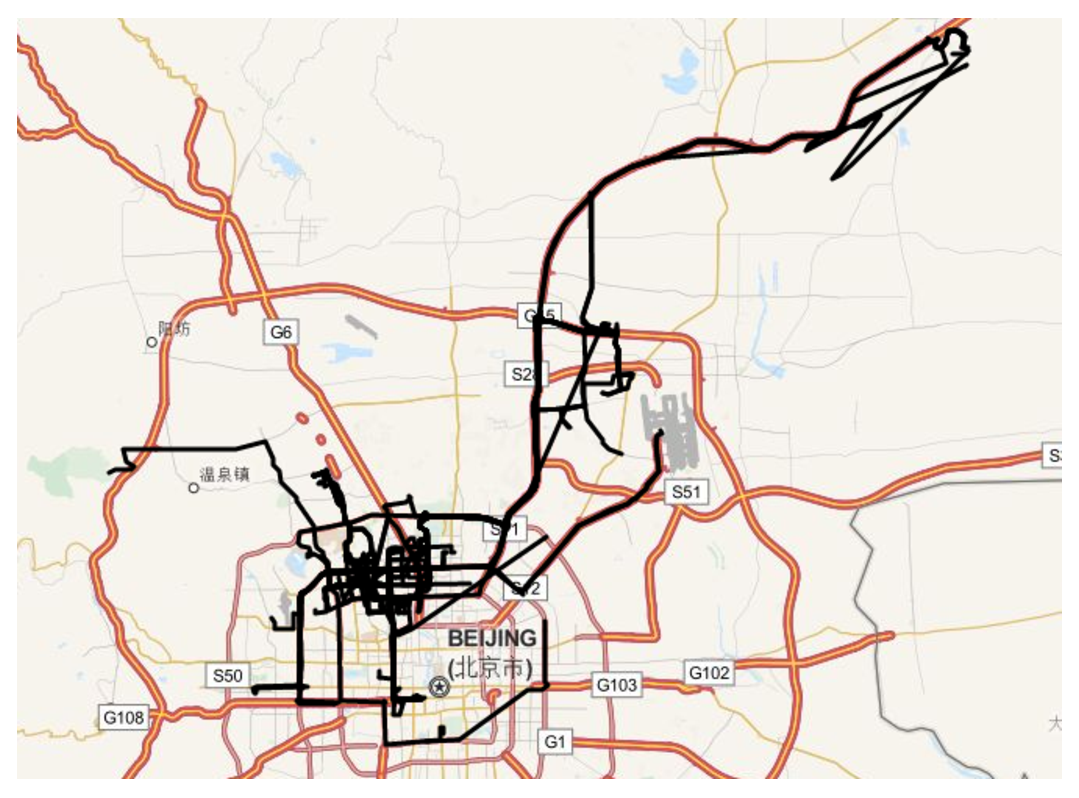
\includegraphics[height=3.6cm]{figs/new/allTrajs.eps}
        \caption{All trajectories of a user}
				\label{fig:allTrajs}
    \end{subfigure}%
		~
    \begin{subfigure}[t]{.15\textwidth}
        \centering
        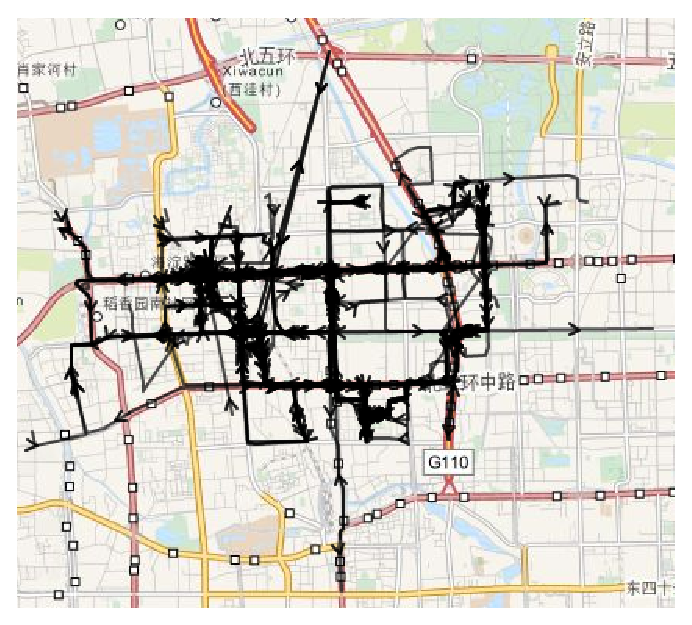
\includegraphics[width=4cm]{figs/dbscn_cluster1.eps}
        \caption{Cluster 1 (227 trajectories)}
    \end{subfigure}%
    }
		\mbox{
    \begin{subfigure}[t]{.2\textwidth}
        \centering
        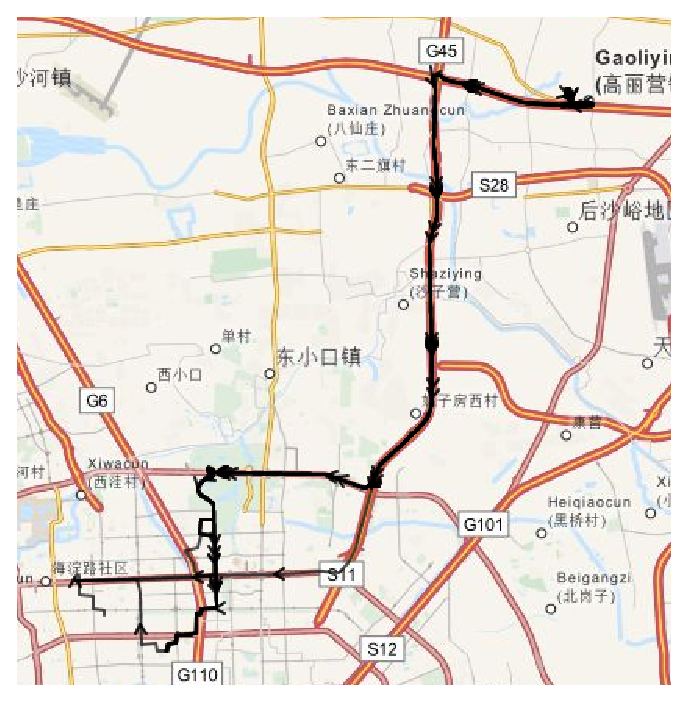
\includegraphics[height=4cm]{figs/dbscan_cluster2.eps}
        \caption{Cluster 2(4 trajectories)}
    \end{subfigure}
    ~
    \begin{subfigure}[t]{.2\textwidth}
        \centering
        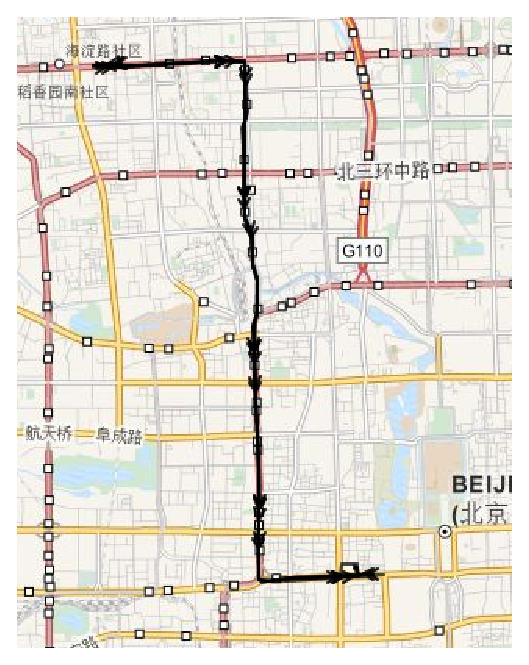
\includegraphics[height=4cm]{figs/dbscan_cluster3.eps}
        \caption{Cluster 3(4 trajectories)}
    \end{subfigure}%
    }
    \caption{Sample user and DBSCAN: Sample user with 323 trajectories. Top summary clusters in DBSCAN summarize user movement poorly}
    \label{fig:DBSCANRes}
\end{figure}
Figure~\ref{fig:DBSCANRes} shows a sample user with 323 trajectories, and the top-3 clusters detected by the DBSCAN with $\UN$ distance metric. We used the \textit{Sorted $k$-dist Graph} methodology proposed in DBSCAN~\cite{ref:dbscan} to compute the optimal values input parameters (which were $\operatorname{minPts}=5$ and $\epsilon=3$ in this scenario). The top cluster has 227 out of 323 trips, and is clearly not summarized user trips well. We tuned the parameters manually to check if we get better clusters. The configuration where $\epsilon=1$ provided better results, but the resulting clusters were not significantly different. 

\paragraph{Hierarchical Clustering}
Hierarchical agglomerative clustering is a bottom-up technique where the algorithm starts by considering each point as a cluster, and merges two `closest' clusters are aggregated to form a higher level cluster. This process is repeated until we reach a single cluster of all points. The definition of closeness of a cluster can be defined in many ways such as complete-linkage, single-linkage or average-link. Hence, Hierarchical clustering forms a tree (usually represented by a dendrogram) where a single cluster of points is repetitively split into two clusters until leaf nodes are reached~\cite{ref:hac}. 

Hierarchical clustering provides the flexibility of analyzing the entire history of user's trajectories, and then cutting the tree at the right level. This enables us to iterate down the tree, and estimate if the sub-tree forms a good cluster based on the distances between the trajectories and other parameters such as the trajectory lengths. We use complete-linkage measure define the distance between two intermediate clusters since it enables us to identify summaries where maximum distance between two trips in the summary is contained.

\subsection{Cluster Identification}
While standard distance metrics and clustering algorithms are well-known, choosing the right metric, clustering algorithm and the parameters for the application is a challenging task. Based on the requires for clustering user trips, we now discuss important approaches and techniques to identify superior summaries. 

Recall that $\UN$ metric is most suited to describe distance between user trips since it provides us an ability to measure the maximum detours between two trips (Section~\ref{sec:trajDist}). Similarly, we motivated the use of hierarchical clustering because of the ability to iterate down the tree, and examine if the trajectories under the tree are similar in terms of trajectory distances and other parameters such as trajectory lengths. 

\begin{figure}
    \mbox{
	 \begin{subfigure}[t]{.2\textwidth}
        \centering
        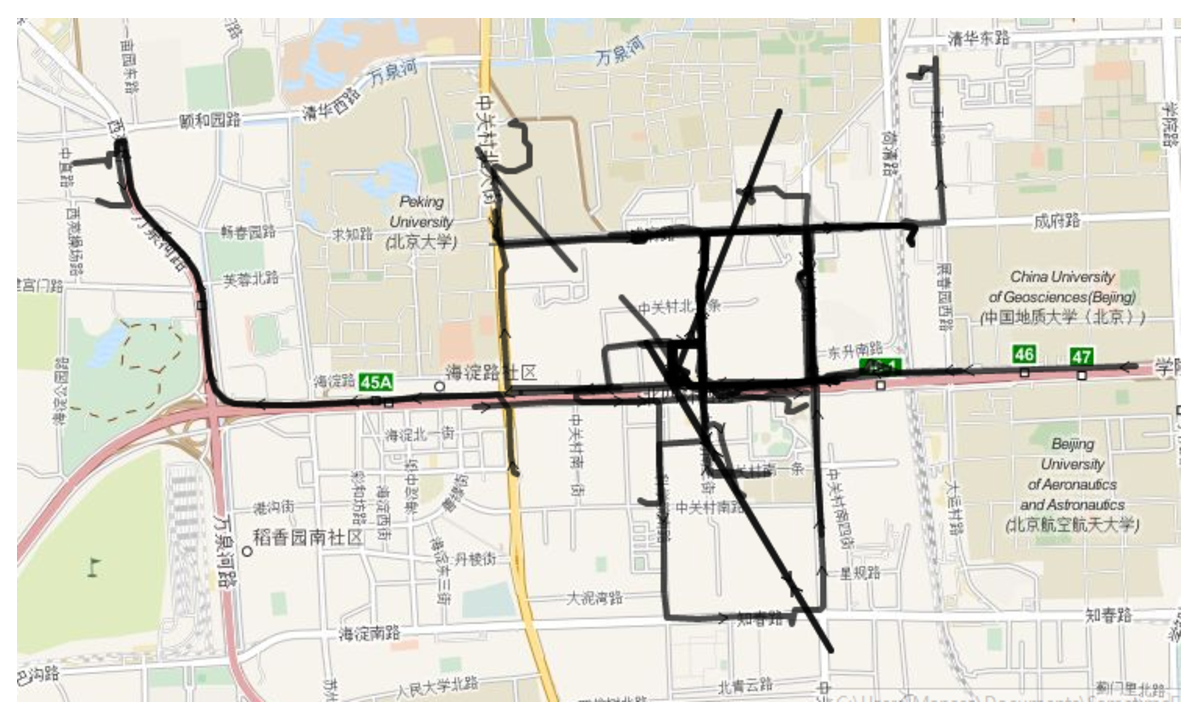
\includegraphics[width=4cm]{figs/new/Elbow_Cluster1.eps}
        \caption{Cluster 1 (32 trajectories)}
    \end{subfigure}%
		~
    \begin{subfigure}[t]{.2\textwidth}
        \centering
        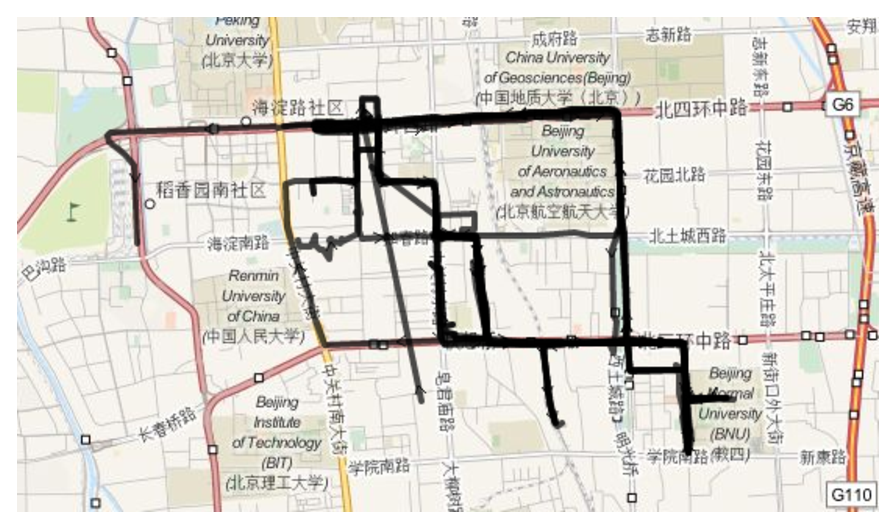
\includegraphics[width=4cm]{figs/new/Elbow_Cluster2.eps}
        \caption{Cluster 2 (31 trajectories)}
    \end{subfigure}
    }
		\mbox{
    \begin{subfigure}[t]{.2\textwidth}
        \centering
        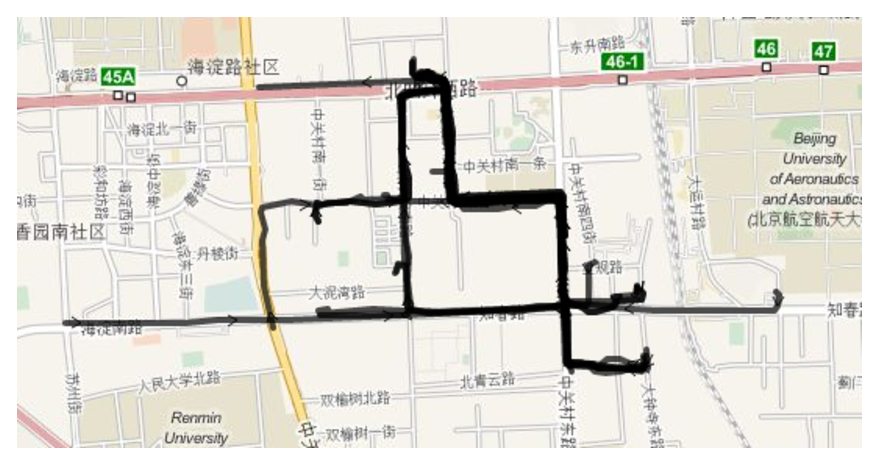
\includegraphics[width=4cm]{figs/new/Elbow_Cluster3.eps}
        \caption{Cluster 3 (31 trajectories)}
    \end{subfigure}%
		\begin{subfigure}[t]{.2\textwidth}
        \centering
        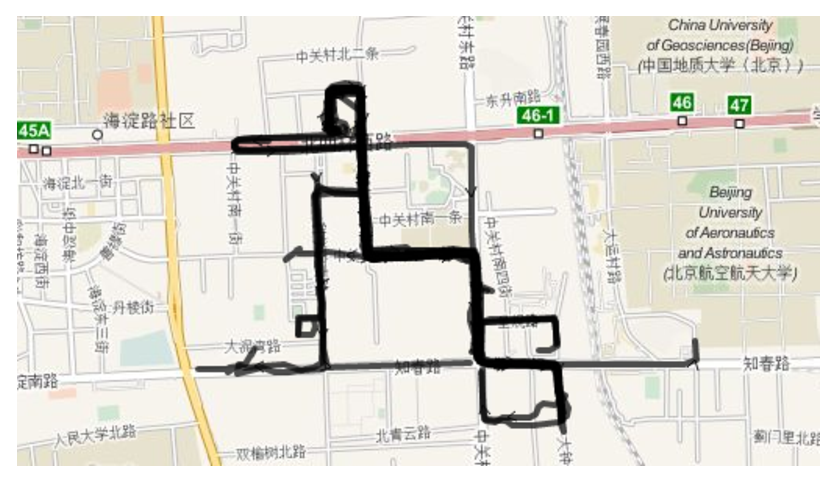
\includegraphics[width=4cm]{figs/new/Elbow_Cluster4.eps}
        \caption{Cluster 4 (31 trajectories)}
    \end{subfigure}
		}
    \caption{Elbow Method: Top-4 summary clusters detected are noisy and unusable}
    \label{fig:elbowVisual}
\end{figure}

Figure~\ref{fig:elbowVisual} shows top-4 clusters detected by the Elbow Method. Clearly, the summaries computed have a lot of dissimilar trips of the user since the elbow point stops at a very low value of $k$.

We first describe well-known Elbow Method to detect optimal number of clusters. Elbow method is widely used in literature to detect the optimal number of clusters for the data-set. Elbow method computes the cumulative \textit{Sum of Squared Errors} (SSE) within the cluster for increasing number of clusters (clusters $k=1,\ldots,N$ having $\operatorname{SSE}=\operatorname{SSE}_1,\ldots,\operatorname{SSE}_N$). SSE decreases as we increase the number of clusters. Elbow method picks the optimal number of clusters as the value of $k$ where the reduction of SSE becomes marginal when compared to reduction in the previous step

The elbow point is determined by plotting $k_i$ vs. $SSE_i$ and picking the $k_i$ which has the largest distance from the line drawn from $SSE_1$ to $SSE_k$. In hierarchical clustering, we can increase $k=1,\dots,N$ by iterating down the tree to find the elbow point.

Identifying the elbow point is non-obvious. We show in Section~\ref{sec:evalSumm} that, in most of the cases, choosing the elbow point results in far inferior summaries; the optimal clusters are far beyond elbow point in most cases. We now propose three new algorithms to identify superior user trip summaries.

\paragraph{\thresh}
\label{sec:thresh}
THRESH is a parametric heuristic to find reasonable clusters of trips. Here, we assume that the analyst can provide a threshold $T$ that signifies the maximum distance between any two trajectories in a cluster (say, \unit{1}{km}). We follow the below steps to identify the trip clusters:
\begin{enumerate}[label=S\arabic*:,topsep=0pt,itemsep=-1ex,partopsep=1ex,parsep=1ex]
\item Compute the distance matrix between trajectories using $\UN$
\item Iterate the dendrogram starting from the root using Breadth-First-Search (BFS).
\item At each node $i$, compute the maximum distance $\operatorname{maxDist}_i$ between all the trajectories under the node $i$. 
\item If the $\operatorname{maxDist}_i < T$, then mark all the trajectories under the node $i$ as a cluster, and delete the sub-tree from node $i$.
\item Else, visit the next node $i$ using BFS. Go to Step 3.
\end{enumerate}

Figure~\ref{fig:threshTopClusters} shows the summary clusters detected by \thresh for the user with trajectories shown in Figure~\ref{fig:allTrajs}. This is clearly superior than the clusters detected by the Elbow Method (Figure~\ref{fig:elbowVisual}) and DBSCAN (Figure~\ref{fig:DBSCANRes})

\begin{figure}
    \mbox{
    \begin{subfigure}[t]{.2\textwidth}
        \centering
        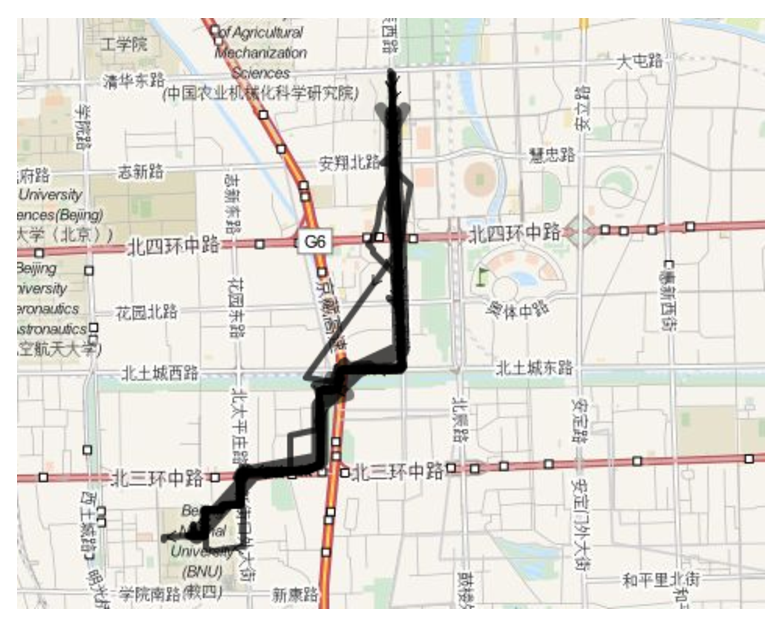
\includegraphics[width=4cm]{figs/new/FinalCluster1.eps}
        \caption{Cluster 1 (20 trajectories)}
    \end{subfigure}%
     
    \begin{subfigure}[t]{.2\textwidth}
        \centering
        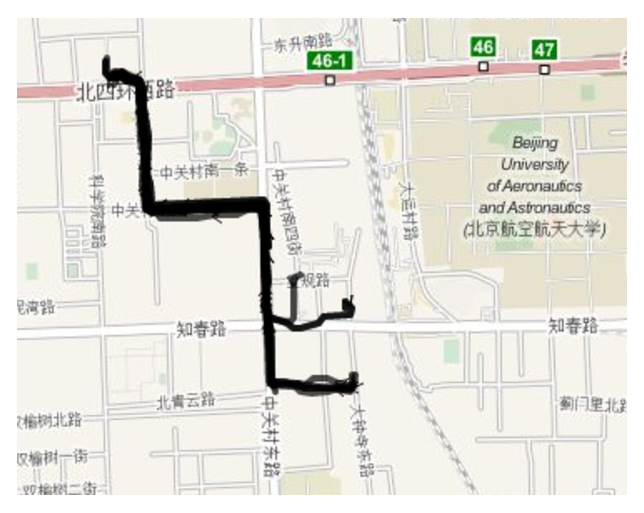
\includegraphics[width=4cm]{figs/new/FinalCluster2.eps}
        \caption{Cluster 2 (15 trajectories)}
    \end{subfigure}
    }
		\mbox{
    \begin{subfigure}[t]{.2\textwidth}
        \centering
        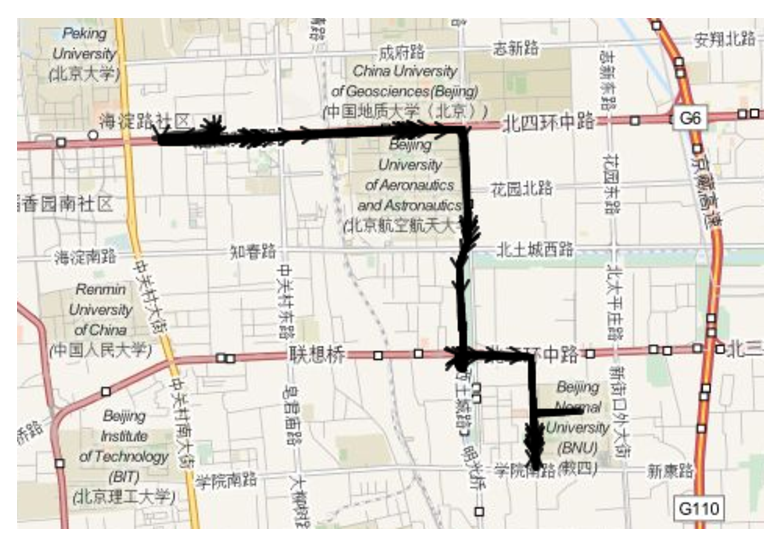
\includegraphics[width=4cm]{figs/new/FinalCluster3.eps}
        \caption{Cluster 3(11 trajectories)}
    \end{subfigure}%
    \begin{subfigure}[t]{.2\textwidth}
        \centering
        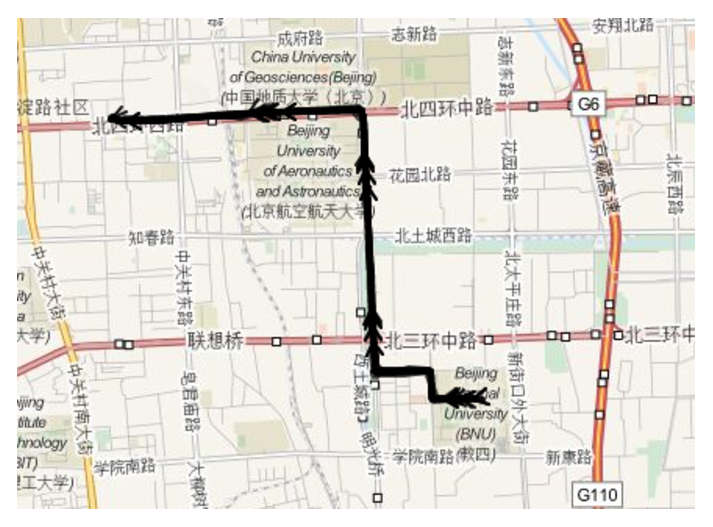
\includegraphics[width=4cm]{figs/new/FinalCluster4.eps}
        \caption{Cluster 4(9 trajectories)}
    \end{subfigure}
		}
    \caption{\thresh: Top-4 summary clusters}
    \label{fig:threshTopClusters}
\end{figure}

\paragraph{\lthAware}
\begin{comment}
\begin{figure}[t!]
\centering
 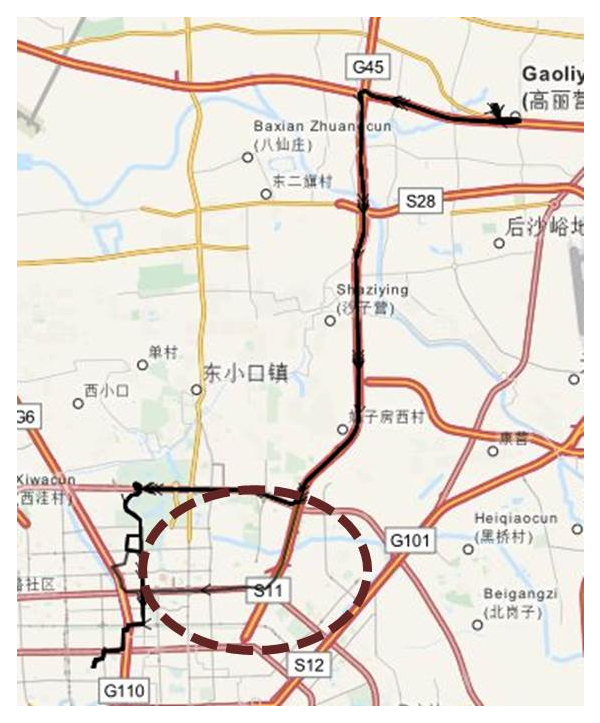
\includegraphics[width=12cm,height=3cm,keepaspectratio]{figs/longtrajs.eps}
 \caption{A cluster with a detour in the middle -- Cluster reported by Modal analysis}
 \label{fig:modal}
 \end{figure}
\end{comment}

Consider a user whose regularly commutes from home to two offices: an office \unit{100}{km} from home and another \unit{5}{km}. Clearly, a deviation of $\unit{1}{km}$ is tolerable while considering the \unit{100}{km} trajectories, and not in the \unit{5}{km} commute trip from home to work. \thresh will be unable to separate these two clusters since it is non-cognizant of the trajectory lengths. We propose a trajectory length aware algorithm \lthAware to overcome this problem. \lthAware operates similar to \thresh algorithm (Section~\ref{sec:thresh}). However, at each node $i$, it computes the trajectory length normalized standardized deviation ($\operatorname{nsd_i}$) as
\begin{align}
	\operatorname{nsd_i}=\frac{\text{std dev of distances between trajectory-pairs under node }i}{\text{mean trajectory length of all trips under node }i}.
\end{align}

The analyst provides a value of tolerable fraction threshold $\operatorname{NSD}$ (say, 0.1 in our case). Steps S4 in \thresh is then changed to the below:
\begin{enumerate}[label=S\arabic*:]
\setcounter{enumi}{4}
\item If the $\operatorname{nsd}_i < \operatorname{NSD}$, then mark all the trajectories under the node $i$ as a cluster, and delete the sub-tree from node $i$.
\end{enumerate}

In Section~\ref{sec:evalSumm}, we show that \lthAware provides a clean separation of trips for users who have regular inter- and intra-city commutes. 

\paragraph{\modal}
\begin{figure*}
\centering
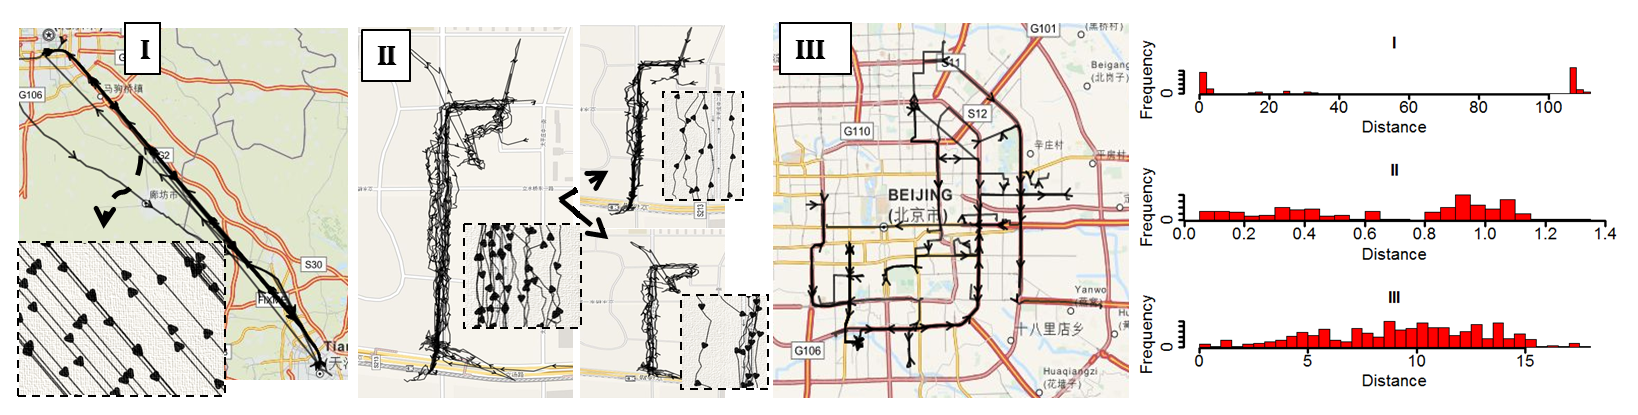
\includegraphics[scale=0.6]{figs/hist_full.eps}
\caption{Illustration of non-parametric nature of MODE-EST: Figs. I and II show the long and short trips. Fig. III shows anomalous cluster. Fig IV shows the bi-modal distribution for Figs. I and II, and unimodal distribution with large mean for Fig. III}
\label{fig:anom}
\end{figure*}

While \lthAware allows trajectory clustering based on the length of the trajectories, it still requires an input parameter that is tuned. We now propose a non-parametric technique that estimates effective clusters without any fixed thresholds. As stated above, standard non-parametric estimates such as Elbow Method do not directly provide good clusters. Hence, we design a technique that examines the distribution of the distances and, based on the number of modes, decides to proceed consider the sub-tree at node $i$ as a cluster or iterate down the tree.

Note that if there are large number of similar trips under a sub-tree at node $i$, then the distance between such trips will be constant, and will appear as a significant mode in the probability density function. We implement the non-parametric test of number of modes using the approach described by Minnotte \textit{et. al.}~\cite{minnotte}. We find the number of modes in the kernel density plot of the pair-wise trajectory distances under node $i$. If there is a single mode, then we accept it as a  cluster of similar trajectories. Else we iterate down the tree. 

However, there is another interesting possibility. The distance distribution under node $i$ might have a single mode, but the distances may be spread out over a very large range. Such a distribution indicates that the trips under node $i$ most probably does not contain any cluster of similar trips; a set of anomalous trips have such characteristics. Hence, we add a post-processing stage to check the condition of anomalous cluster: if there is a single mode and the mean of pair-wise trajectory distances is greater than some large distance $L$. If such anomalous cluster condition is detected, then we prune out the node $i$ without accepting the underlying trajectories as a cluster of similar trajectories. This also saves computation time since we do not iterate down the sub-tree.

We now illustrate the modes and the distance distribution in our dataset. Figure~\ref{fig:anom} (I and II) shows the bi-modal distribution of long inter-city trajectories between Beijing and Tianjin (\unit{135}{km}) and short intra-city (\unit{1}{km}) trips, where the to- and fro-trips have different distances between each other. Figure \ref{fig:anom} III shows an anomalous cluster detected with the corresponding histogram of distances.

% Final summary
In all the above schemes, we finally represent the ``Summary Clusters'' of a user as the clusters with number of trajectories greater than a certain threshold (5\% of user's trajectories in our case)

\begin{comment}
\subsection{Finding optimal clusters}
Number of clusters in the summary: Since each person's movement is unique(?), the number of clusters and the number of trajectories expected in each clusters are not constant. Hence, standard mechanisms such as k-means clustering cannot be directly applied to summarize. Even after the clusters are found out, we need to see if this cluster represents points that have meaningful end-to-end trips.% \rednote{This is not coming out good. Need to think}
We need good OD +  we need trajectories that are not far away in the middle. One way to design a sim metric that is cognizant of: (1) origins, destinations, directionality and (2) the maximum separation between the trajectories. However, such a sim metric will introduce other artifacts (say, by classifying far away trajectories into same cluster). Hence we consider an approach where we decouple by considering O/D and direction in the sim metric, and then design an algorithm to select optimal number of clusters by looking at the maximum intra-cluster separation.
\end{comment}

\subsection{Representative trajectories}
\label{sec:repTraj}
We now find a representative trajectory for each of the cluster that can be used as a proxy for a Summary Cluster. One approach is to consider the mean trajectory curve $\meanTraj_i$ as a representative for the cluster $\summClus_i$. However, since the mean of multiple curves may not fall on any of the individual trajectories (and hence the roads on which the user went), it is not recommended as a representative. Hence, we follow a well-known method of computing piece-wise median trajectories~\cite{median1}. Here, at an interval of $\delta$ number of points on interpolated mean trajectory, one point on any of the trajectories in the cluster closest to the mean is added to the representative trajectory. 

\begin{comment}
\subsection{Storing the trajectories at various levels of granularity}
\subsection{Intra-cluster Movement Pattern}
\end{comment}

\begin{comment}
Similarity metric for summarizing human movement should consider the below aspects
\begin{itemize}
\item Importance to Origins and Destinations: Hurricanes and other physical effects (?) are generally governed by physical laws and computing similarity might have to account for different effects. However, movement of a people is generally associated with an intention (such as commuting to work) of moving from an origin point to a destination point. Hence, a reasonable summary of a person's movement accounts for end-to-end trips that she takes. Currently, there is no similarity metric that gives any bias to the endpoints of the trajectory. We try to plug the bias into our similarity metric so that trip intentions are also given importance. 
For example, SWARM does not consider explicitly consider the end points of the trajectory. Hence, it might wrongly categorize movement on similar roads -- even with varying end points -- into the same cluster. %\rednote{Show a toy scenario that shows how SWARM has mistook two different o-d clusters to be in the same cluster}

\item Metric: Clustering trajectories using standard clustering algorithms require the distance function between two trajectories to be a mathematical metric. In the current literature, only a few functions are metrics \cite{lp,edwp}. Others, which mostly take care of artifacts of sampling, are shown to be non-metrics. Using such functions, which violate properties like triangular inequality, in clustering can lead to unforeseen results. %\rednote{Show a figure where tri inequality is violated in actual sense}
Ex of triangle inequality - User 014 ; Trajs 3,11,175;
3-175(124)>3-11(94)+11-175(4.283)

\item Sampling artifacts: Is time stretching and shrinking important? Are sampling points important? Ours is better because we consider human specific movement where direction and OD are important. While sampling frequency and alignment of samples is required, more or less all traces can be preprocessed after good samples have been taken. So, it really doesnt make sense to consider the effect of timing of samples (like DTW) while designing the clustering algorithm. %\rednote{Vinay: Show a toy scenario where DTW goes wrong}
\end{itemize}

\paragraph{Origin-Destination}
In human movement, similar trips are usually between similar origin and destination regions. For example, the summary of a vast majority of working population are their trajectories between home and office. Hence, the similarity function should provide greater importance to OD. We define \textit{Weighted LP-Norm for OD} as
\begin{align}
w_{\od}(t, c, r) &= 
	\begin{cases} 
		\frac{c}{r} &\mbox{if } t \le \frac{r}{2} \mbox{ or } t > (1 - \frac{r}{2}), \\ 
		\frac{1- \frac{c}{r}}{(1-r)} & \mbox{otherwise},
	\end{cases}
\end{align}
\noindent where $r$ and $c$ denote the parameters define the weight assigned to the origin and destination stretches when compared to the intermediate stretch. Here $r$ defines the fraction of the stretch from origin or towards destination which has to be given a prominence ($r=[0,1]$). And, $c$ is the weight assignment factor at O and D stretches ($c=[0,1]$). If $c > 1 -r$, then the origin and destination stretches of length $\frac{r}{2}$, will be given a higher weight than the intermediate stretch (of length $1 - r$)


\noindent
For Uma's work:
Let $x_i \ge 0$ represent the ``color of grid $i$''. \\
Let $N(i) = \left \{ \text{All grids that are neighbors of i} \right \}$. \\
Let $C$ be the ``conflicting set''. A tuple $(i,j)$ is added to the conflicting set $C$ if two grids $i$ and $j$ have a \textit{LAC separating line} between them.\\
Let $y_i$ be an indicator variable to say if the grid has same color as at-least one of its neighbor.

We formulate an optimization problem to find the color for each grid as below:
\begin{align}
\mbox{Min} \sum_{i}{y_i}
\end{align}
\noindent such that:
\begin{align}
x_i &\neq x_j, ~~~\forall (i,j) \in C\\
y_i &= 
\begin{cases} 
		1 &\mbox{if } \forall j=N(i), x_i = x_j, \\ 
		0 &\mbox{otherwise}.
	\end{cases}
\end{align}

In order to assign similarity scores  to pairs of trajectories, we first have to resample them into equal number of points. 
\paragraph{Resampling and Interpolation}
\paragraph{Using Linear Interpolation over Spline}
%\rednote Image showing problems when using spline interpolation 
\begin{figure}
\centering
\includegraphics[scale=0.4]{figs/spline.jpg}
\caption{Problems with spline interpolation}
\label{fig:spline}
\end{figure}
\paragraph{Resampling and then applying DTW is very close to using our similarity measure }
\end{comment}
\section{Evaluation and Analysis}

\subsection{Dataset}
\begin{itemize}
\item Microsoft GeoLife Dataset
GeoLife Dataset published by Microsoft Research \cite{geolife1},\cite{geolife2},\cite{geolife3}. This is a GPS trajectory dataset with GPS traces of 182 users over a period of three years (from April 2007 to August 2012). 
\item Microsoft T Drive Taxicab Dataset
This is a trajectory dataset that contains one-week trajectories of 10,357 taxis published by Microsoft Research. \cite{tdrive1} ,\cite{tdrive2}
\end{itemize}
\subsection{Clustering Effectiveness}
We have shown various comparisons and result, but the main measure of clustering effectiveness that we use is the Silhouette Coefficient(SC). SC is a standard metric that shows the effectiveness of clustering. SC is based on the cohesion and the separation of clusters formed. The cohesion ( \textit{a(x)})  is defined as the average distance of x to all other vectors in the same cluster. 
The separation (\textit{b(x)}) is defined as the minimum of the average distances of x to the vectors in other clusters.
Further, the silhouette coefficient of a data point is defined as 
\begin{equation}
s(x)=\frac{b(x)-a(x)}{max(a(x),b(x))}
\end{equation}
The total silhouette coefficient of the dataset is the average over all the points given by
\begin{equation}
SC=\frac{1}{N}\sum_{i=1}^{N}s(x)
\end{equation}
\noindent Ideally, SC is between [-1,1], where values closer to 1 representing better formed clusters. 

\subsection{Individual Movement Summary}

In this section, we talk about the experiments made on the Microsoft GeoLife Dataset. These are GPS traces of around 182 users collected over a period of three years. From this data, we aim at finding the movement summary of the person which will give us insights into how that person moves and which patters appear repeatedly. In the first section we show the working of our proposed method with supporting visuals at every step explaining the rationale behind it. Further, we implemented and modified some other works from the literature to suit the problem and have discussed the results. A brief description of the methods we have compared with are given below.

\paragraph{Dynamic Time Warping}
This is a comparison made in the choice of the similarity metric that we use. We show the effects of using DTW in place of our similarity measure, keeping everything else in the algorithm exactly as it is.The DTW similarity between A and B is defined below 
\begin{equation}
D_{dtw}(A,B) =
\left\{
	\begin{array}{ll}
		0  & \mbox{if } \text{both A and B are empty} \\
		\infty & \mbox{if } \text{one of A or B is empty}\\
                \phi _d (head(A),head(B))+
                   \\min 
\left\{
	\begin{array}{ll}
		D_{dtw}(A,rest(B)), \leftarrow \text{\emph{Stretch A}}\\

		D_{dtw}(rest(A),B),\leftarrow \text{\emph{Stretch B}}\\
                D_{dtw}(rest(A),rest(B)) 
	\end{array}
\right.          \\otherwise
	\end{array}
\right.
\end{equation}

where $\phi_d(p1,p2)=L_2-dist(p1,p2)$ 
\paragraph{SWARM}
SWARM is a moving objects clustering algorithm proposed by Li \emph{et al.}\cite{Li2010}  In this algorithm they consider trajectories to be of the same cluster if they are together in similar clusters for a specific number of (not necessarily consecutive) timestamps. 
\paragraph{TRACLUS}
 TRACLUS is an algorithm proposed by Lee \emph{et al.} in \cite{Lee2007}. This algorithm partitions the trajectories, clusters the partitions and then comes up with a final representative cluster. 


\subsubsection{Proposed Method-OD}
In this section we show each stage of the proposed method and the corresponding visualizations at that stage for a test user. 
Fig. \ref{fig:alltrajs} shows all the trajectories of the user. We compute the similarity matrix using the similarity defined earlier  and run hierarchical clustering on it. 

\begin{figure}
\centering     
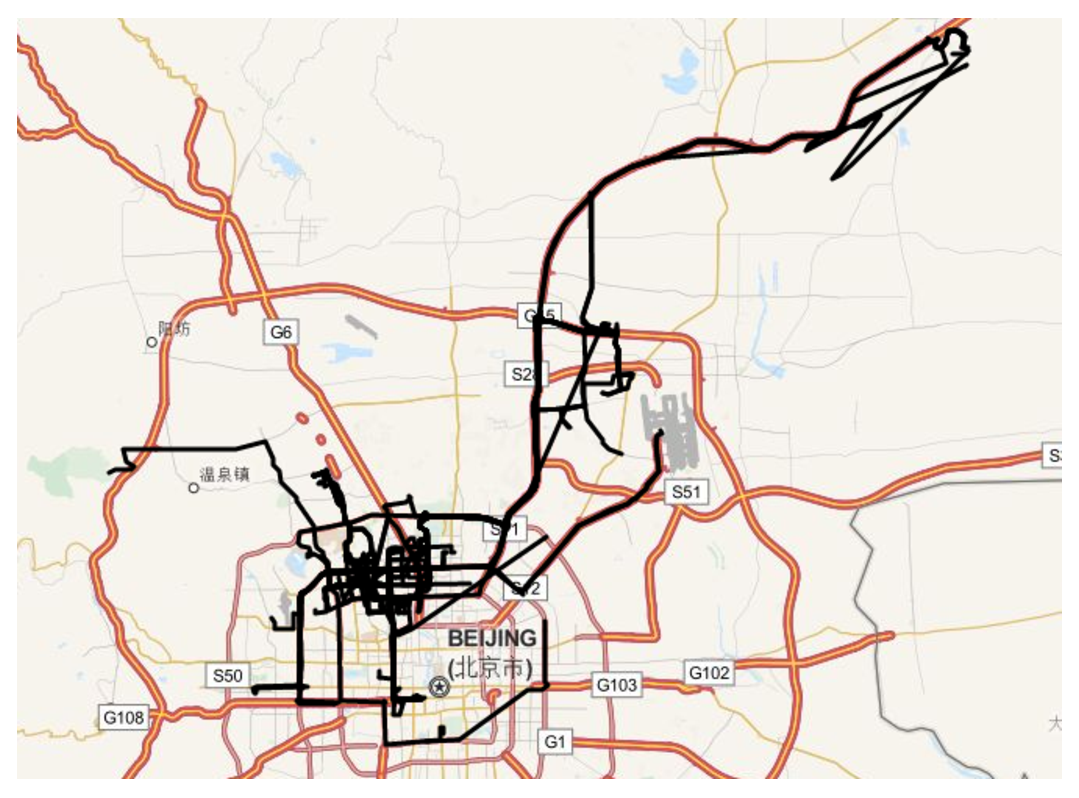
\includegraphics[scale=0.4]{figs/new/allTrajs.eps}
\caption{A snapshot of all the trajectories of the test user (363 trajectories in total)}
\label{fig:alltrajs}  
\end{figure}


The dendrogram is a pictoral representation of how similar the trajectories are among each other. The ones more similar to each other are paired closer to the bottom as compared to the ones higher in the tree. Fig \ref{fig:dendrogram} shows the dendrogram of the trajectories of the test user. The user had 363 trajectories in total, so the dendrogram has 363 leaves. 
\begin{figure}[t]
\centering     
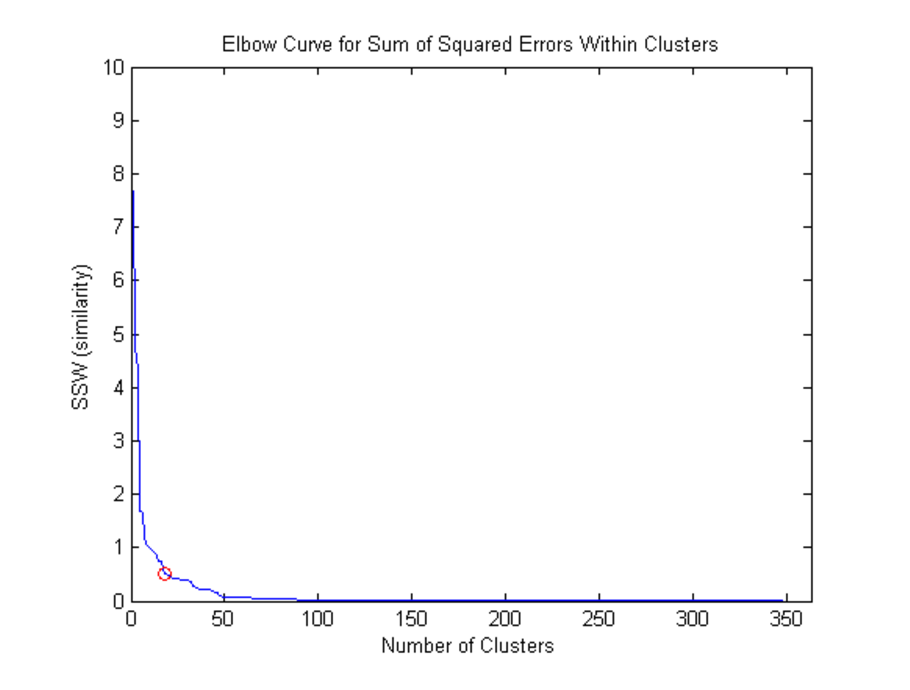
\includegraphics[scale=0.5]{figs/new/elbow.eps}
\caption{Elbow curve - Plot of the SSW vs number of Clusters; Elbow point ~ 18 clusters}
\label{fig:elbow}  
\end{figure}
\begin{figure*}
\centering     
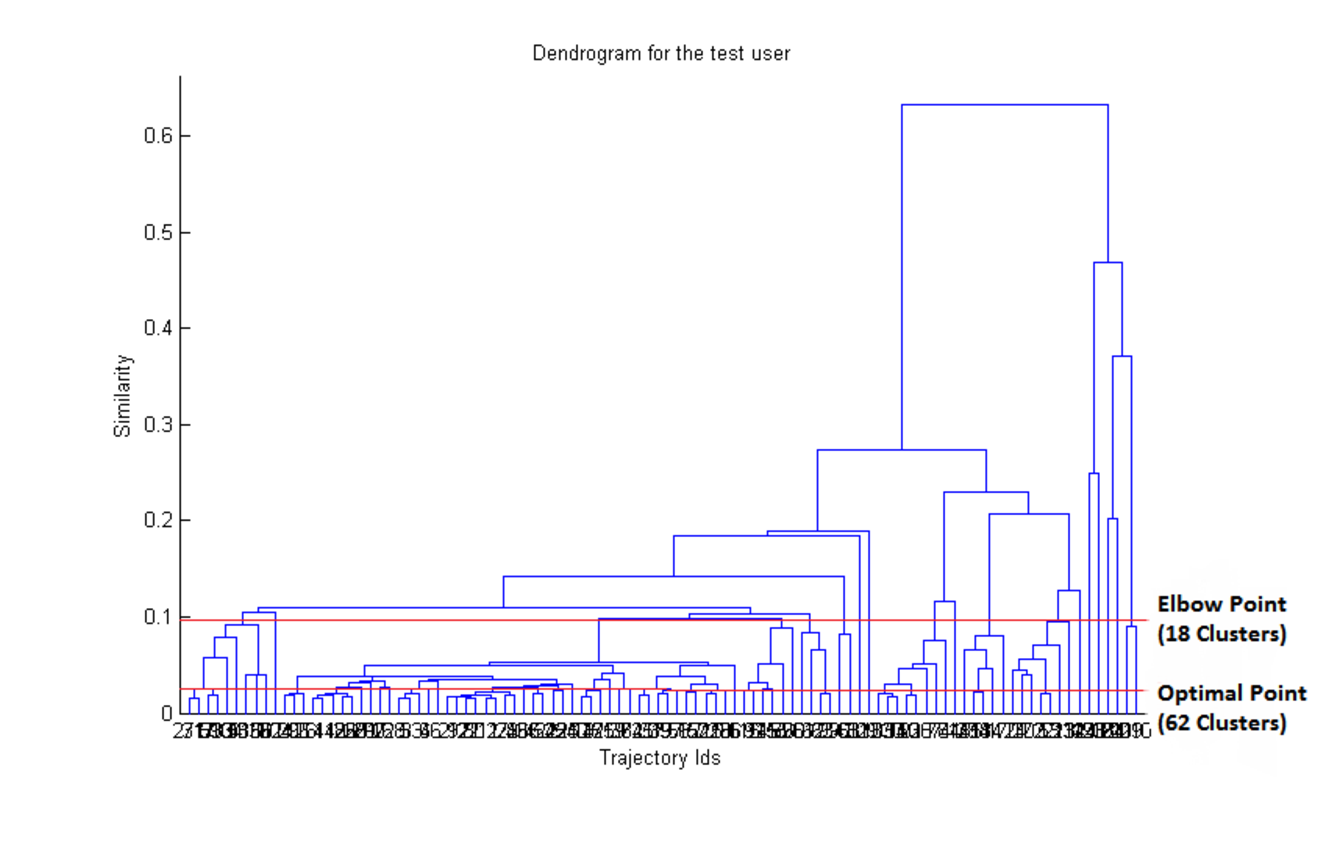
\includegraphics[scale=0.5]{figs/new/dendrogram.eps}
\caption{Dendrogram of the all the trajectories (Shows the hierarchy of similarity) The elbow point is at 18 clusters, whereas the optimal number of clusters is 62 }
\label{fig:dendrogram}  
\end{figure*}
To obtain a certain cluster of the trajectories, we have to cut the dendrogram at a certain level. The height at which we cut the dendrogram decides the number of clusters we will get. Finding the right height at which we should cut the dendrogram is one of the biggest challenges in coming up with an accurate summary for a user. One method which is widely used in literature is to plot the cumulative Sum of Squared Errors within Cluster as the cluster number varies from 1 to N. This is called the elbow curve or the scree plot and the elbow point in this curve should give us the right number of clusters. The rationale behind this is that we want to find the saturation point beyond which even on increasing the number of clusters, the error within the clusters doesnt decrease significantly. But, in our case, we found that the elbow point doesn't get us anywhere close to the actual optimal point of clustering. The validation of the clusters formed at each value of number of clusters was done by visualizing the results and looking at the general tightness of the clusters. Fig \ref{fig:elbow} shows the elbow curve with two lines indicating the elbow point, and the optimal cluster number. We see that the actual optimal point is way beyond the elbow point, and show the visualizations of the top 4 clusters at both the elbow point, in Fig. \ref{fig:elbowVisual} and (elbow point +5) number of clusters in Fig. \ref{fig:elbow5visual}.  


\begin{figure*}
    \centering
    \begin{subfigure}[t]{.5\textwidth}
        \centering
        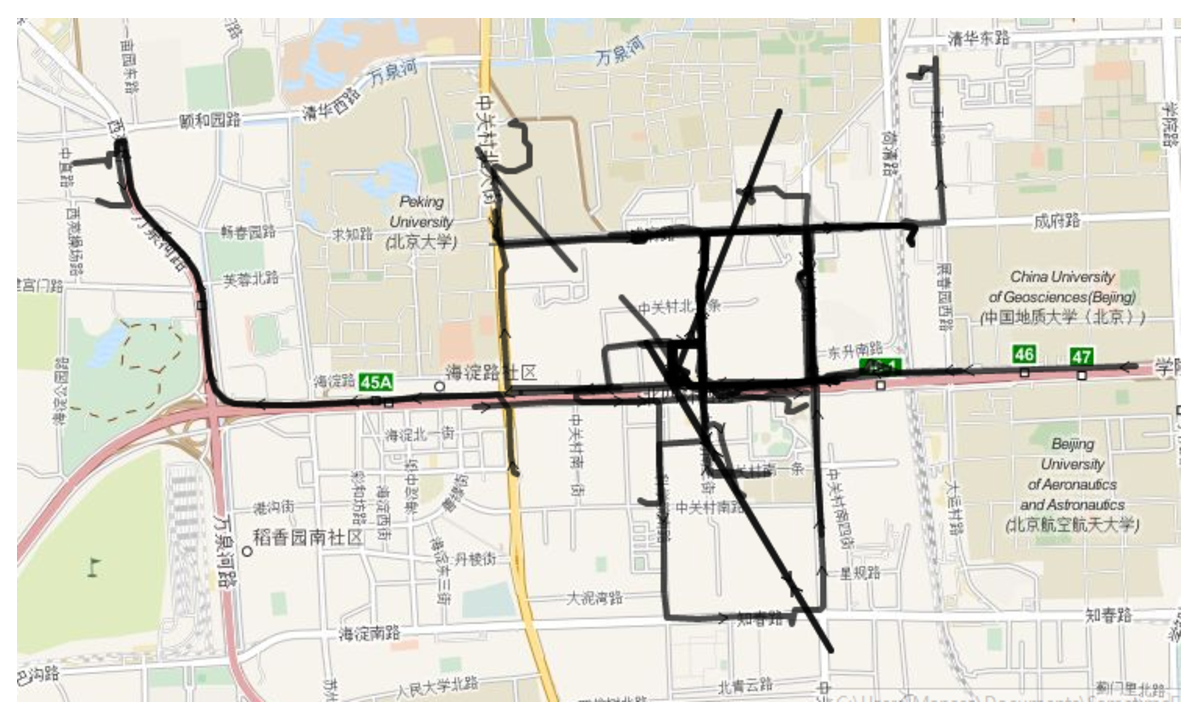
\includegraphics[width=6cm,height=4cm,keepaspectratio]{figs/new/Elbow_Cluster1.eps}
        \caption{Cluster 1 ( 32 trajectories)}
    \end{subfigure}%
    \begin{subfigure}[t]{.5\textwidth}
        \centering
        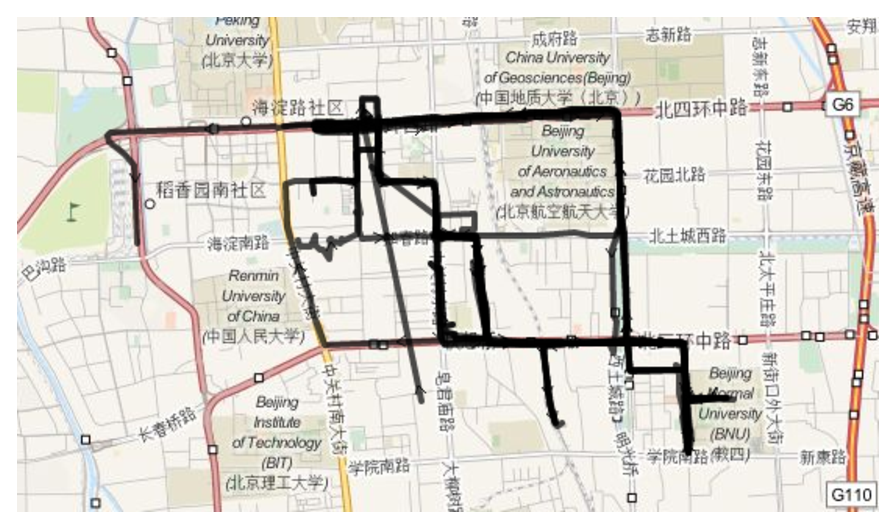
\includegraphics[width=6cm,height=4cm,keepaspectratio]{figs/new/Elbow_Cluster2.eps}
        \caption{Cluster 2(31 trajectories)}
    \end{subfigure}
        
    \begin{subfigure}[t]{.5\textwidth}
        \centering
        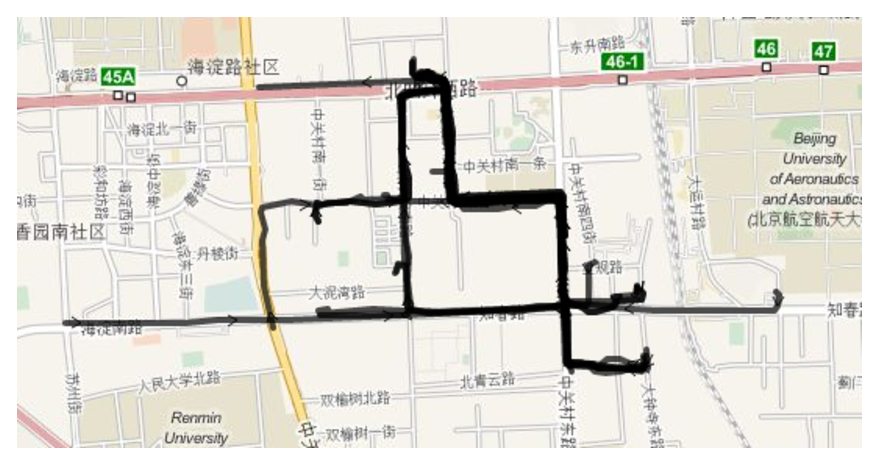
\includegraphics[width=6cm,height=4cm,keepaspectratio]{figs/new/Elbow_Cluster3.eps}
        \caption{Cluster 3(31 trajectories)}
    \end{subfigure}%
    \begin{subfigure}[t]{.5\textwidth}
        \centering
        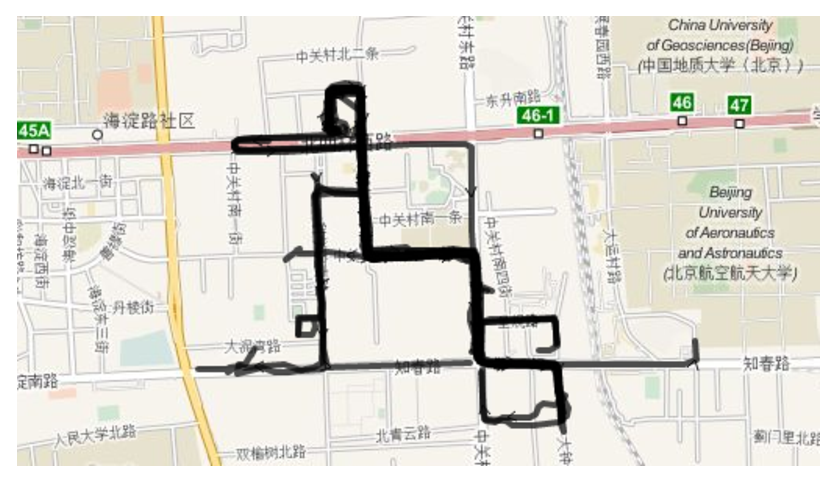
\includegraphics[width=6cm,height=4cm,keepaspectratio]{figs/new/Elbow_Cluster4.eps}
        \caption{Cluster 4(31 trajectories)}
    \end{subfigure}
    \caption{Visualizations of the top 4 clusters at Elbow Point}
    \label{fig:elbowVisual}
\end{figure*}

\begin{figure*}
    \centering
    \begin{subfigure}[t]{.5\textwidth}
        \centering
        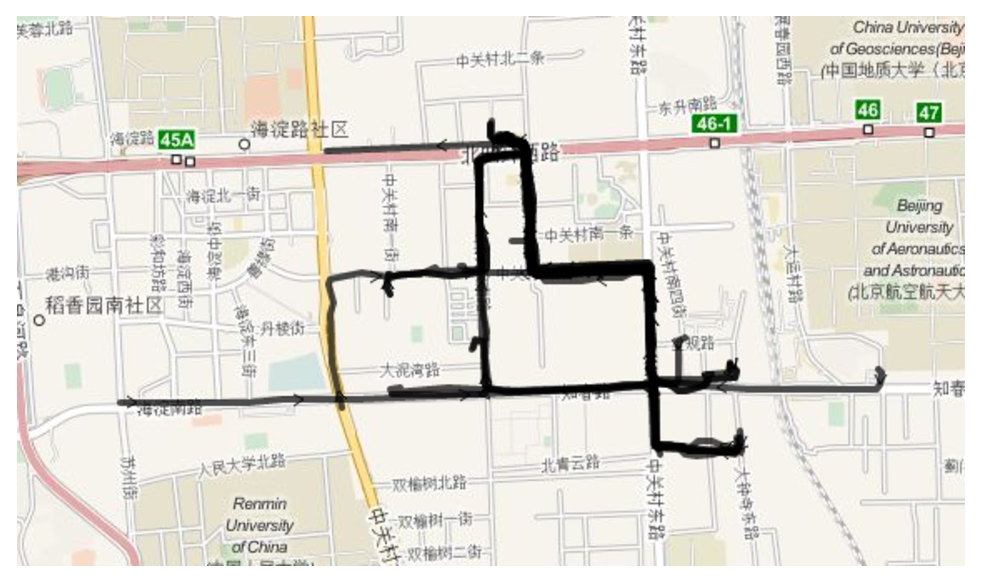
\includegraphics[width=6cm,height=4cm,keepaspectratio]{figs/new/Elbow5_Cluster1.eps}
        \caption{Cluster 1 ( 31 trajectories)}
    \end{subfigure}%
    ~ 
    \begin{subfigure}[t]{.5\textwidth}
        \centering
        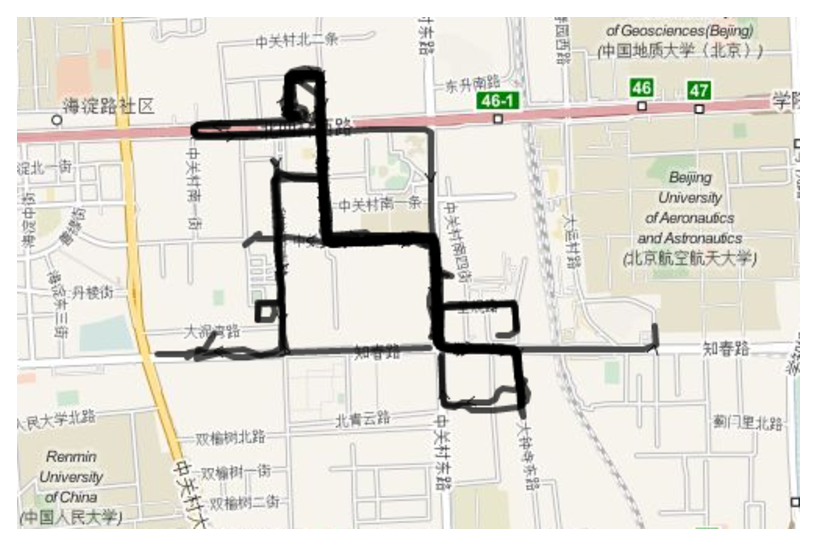
\includegraphics[width=6cm,height=4cm,keepaspectratio]{figs/new/Elbow5_Cluster2.eps}
        \caption{Cluster 2(31 trajectories)}
    \end{subfigure}
    
    \begin{subfigure}[t]{.5\textwidth}
        \centering
        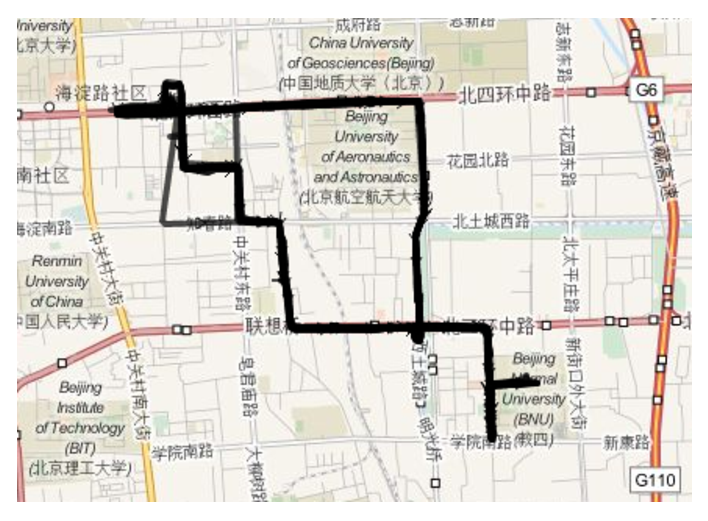
\includegraphics[width=6cm,height=4cm,keepaspectratio]{figs/new/Elbow5_Cluster3.eps}
        \caption{Cluster 3(24 trajectories)}
    \end{subfigure}%
    \begin{subfigure}[t]{.5\textwidth}
        \centering
        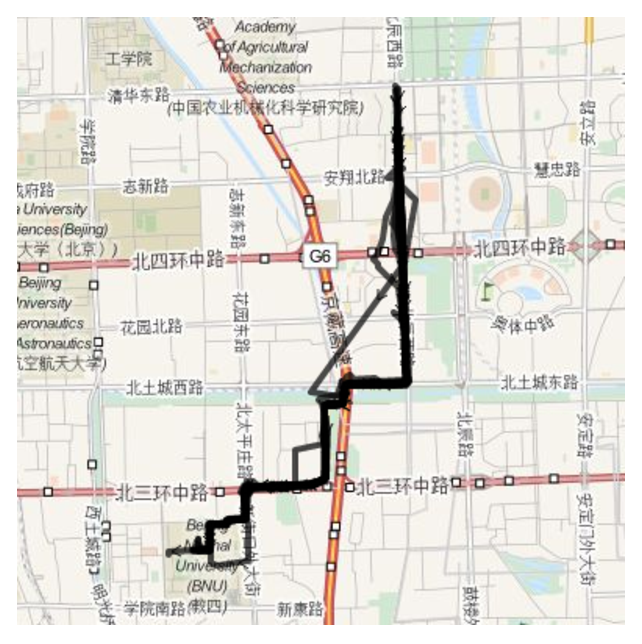
\includegraphics[width=6cm,height=4cm,keepaspectratio]{figs/new/Elbow5_Cluster4.eps}
        \caption{Cluster 4(20 trajectories)}
    \end{subfigure}
    \caption{Visualizations of the top 4 clusters at Elbow Point+5 point- Clusters not tight enough,need to go down the dendrogram further}
    \label{fig:elbow5visual}
\end{figure*}
Thus, we see that the elbow point does not get us anywhere close to the optimal number of clusters, but can help as a starting point for finding the optimal number. One insight that the elbow point gives is that the optimal point cant be before the elbow point, and hence we can prune the search space till the elbow point. 
The heuristic that we follow to obtain the optimal number of clusters is to traverse down the dendrogram , starting from the elbow point, and at any stage if we hit a cluster where the maximum pointwise distance between any pair of trajectories is less than $\delta$, we report it as a final cluster. 
\begin{figure*}
    \centering
    \begin{subfigure}[t]{.5\textwidth}
        \centering
        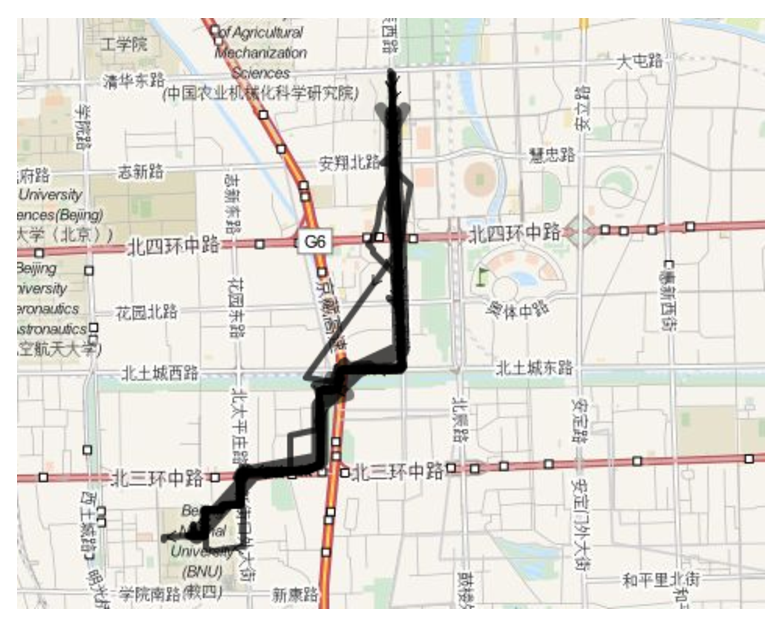
\includegraphics[width=6cm,height=4cm,keepaspectratio]{figs/new/FinalCluster1.eps}
        \caption{Cluster 1 ( 20 trajectories)}
    \end{subfigure}%
    ~ 
    \begin{subfigure}[t]{.5\textwidth}
        \centering
        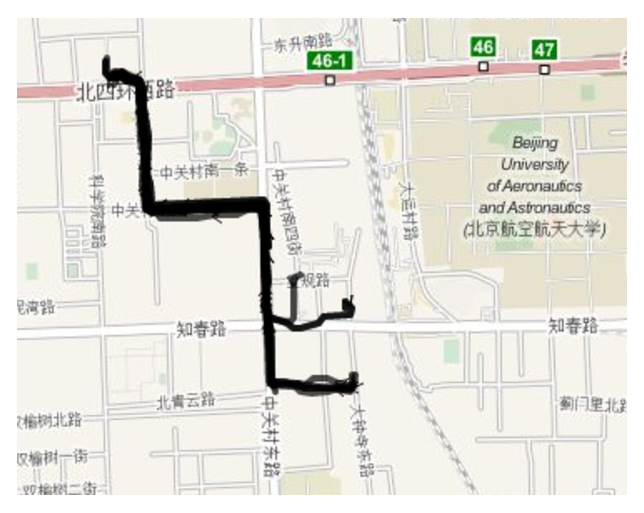
\includegraphics[width=6cm,height=4cm,keepaspectratio]{figs/new/FinalCluster2.eps}
        \caption{Cluster 2(15 trajectories)}
    \end{subfigure}
    
    \begin{subfigure}[t]{.5\textwidth}
        \centering
        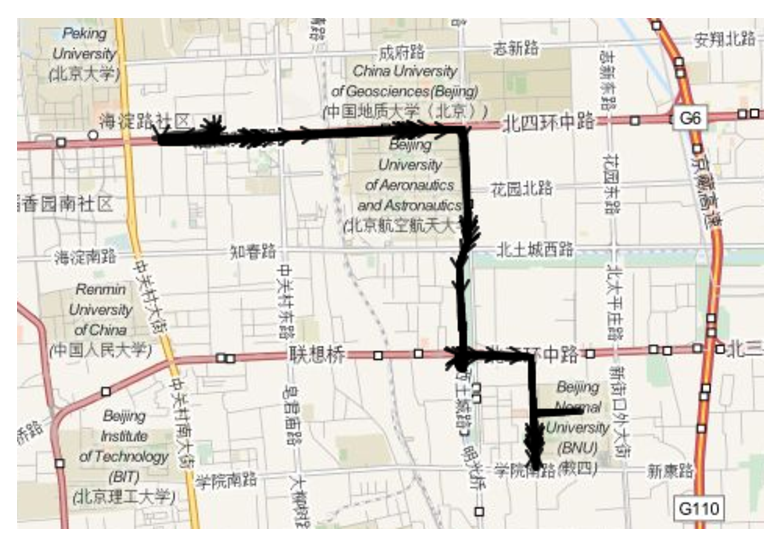
\includegraphics[width=6cm,height=4cm,keepaspectratio]{figs/new/FinalCluster3.eps}
        \caption{Cluster 3(11 trajectories)}
    \end{subfigure}%
    \begin{subfigure}[t]{.5\textwidth}
        \centering
        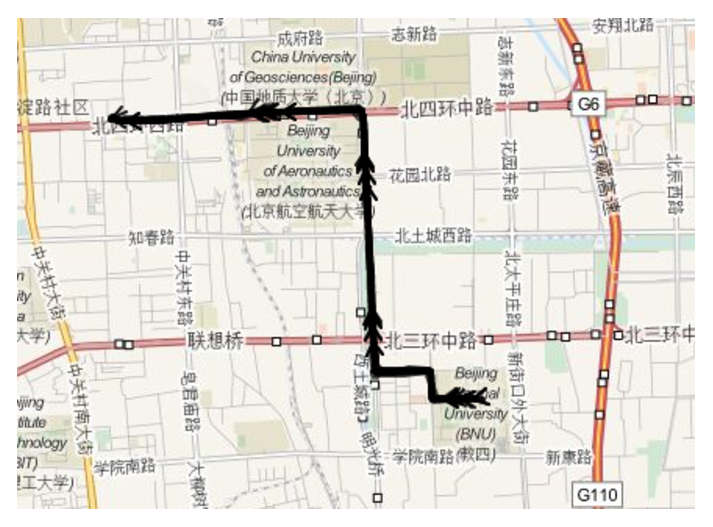
\includegraphics[width=6cm,height=4cm,keepaspectratio]{figs/new/FinalCluster4.eps}
        \caption{Cluster 4(9 trajectories)}
    \end{subfigure}
    \caption{Visualizations of the top 4 final optimal clusters}
    \label{fig:finalClusters}
\end{figure*}

Fig.\ref{fig:finalClusters} shows the visualizations of the top-4 clusters at the optimal level. 
\subsubsection{Variation with DBSCAN} 
In order to make an attempt at doing away with the heuristic, we tried another approach. In this approach we perform two stages of clustering followed by a DBSCAN based on the OD similarity measure we proposed. This method is described below : 
\begin{itemize}
\item In the first stage, we cluster the trajectories based on the Origin to origin distance. We run hierarchical clustering, and then plot the elbow curve for the SSW values and cluster it at the elbow point. 
\item In the next stage, we further cluster each cluster obtained from above based on the destination distances and performing hierarchical clustering individually on each of the clusters.
\item Once we have performed the origin and destination clusters, we now have trajectories clustered on their OD values. Now, on each of these individual clusters, we run DBSCAN based on the similarity proposed earlier. The values for minLns and epsilon are chosen using the heuristic mentioned in the paper .
\end{itemize}
By using this variant, we dont use the heuristic at any step, and are still successful in getting optimum results. The visualizations of the top 4 clusters by using this method is shown in Fig. \ref{fig:DBSCANRes}
\begin{figure*}
    \centering
    \begin{subfigure}[t]{.5\textwidth}
        \centering
        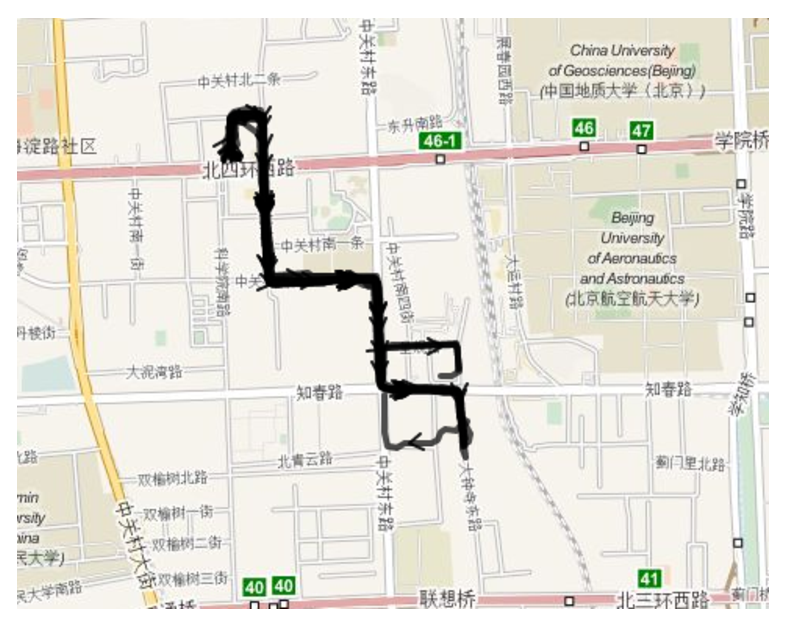
\includegraphics[width=6cm,height=4cm,keepaspectratio]{figs/new/DBSCAN1.eps}
        \caption{Cluster 1 ( 19 trajectories)}
    \end{subfigure}%
    ~ 
    \begin{subfigure}[t]{.5\textwidth}
        \centering
        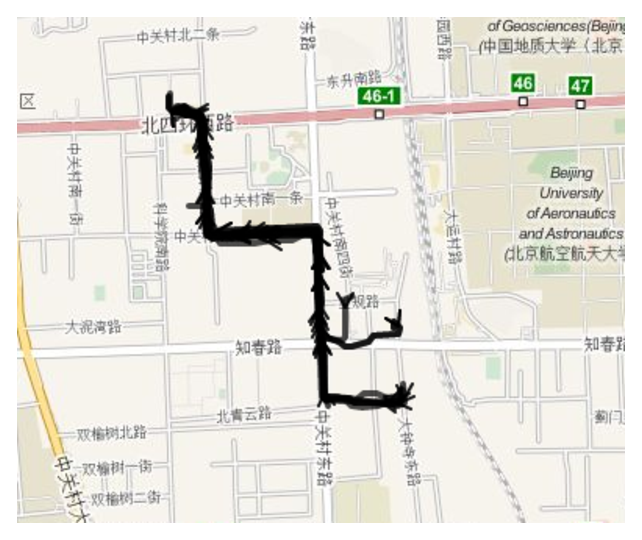
\includegraphics[width=6cm,height=4cm,keepaspectratio]{figs/new/DBSCAN2.eps}
        \caption{Cluster 2(16 trajectories)}
    \end{subfigure}
    
    \begin{subfigure}[t]{.5\textwidth}
        \centering
        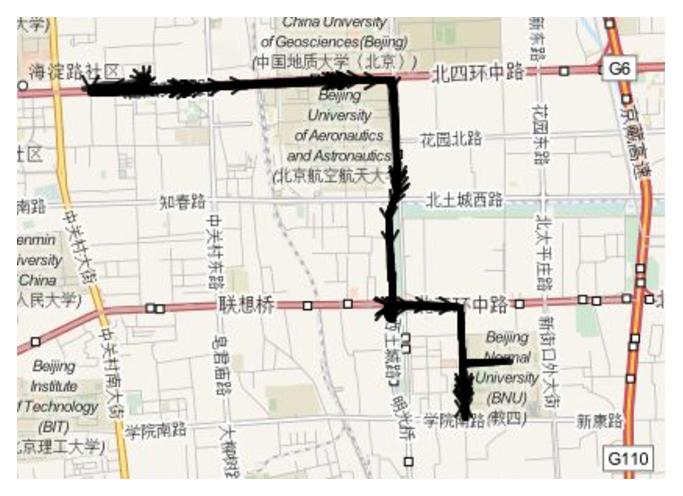
\includegraphics[width=6cm,height=4cm,keepaspectratio]{figs/new/DBSCAN3.eps}
        \caption{Cluster 3(11 trajectories)}
    \end{subfigure}%
    \begin{subfigure}[t]{.5\textwidth}
        \centering
        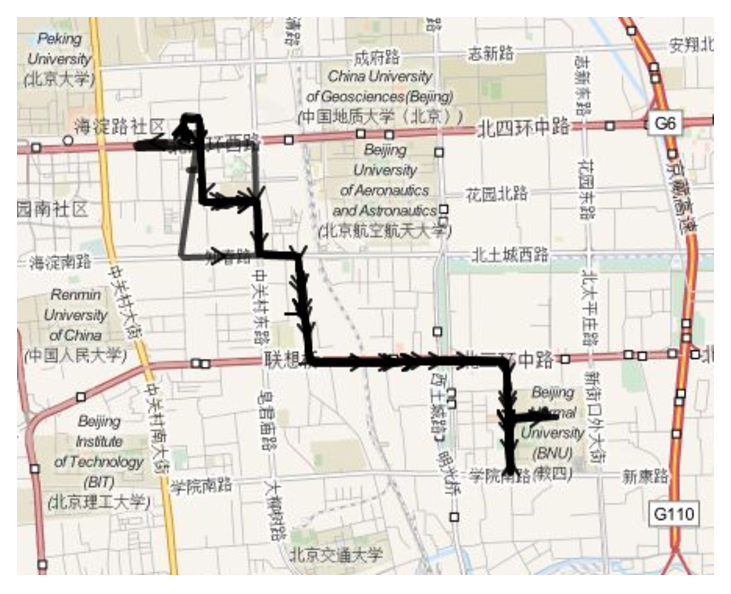
\includegraphics[width=6cm,height=4cm,keepaspectratio]{figs/new/DBSCAN4.eps}
        \caption{Cluster 4(9 trajectories)}
    \end{subfigure}
    \caption{Visualizations of the top 4 final optimal clusters using the DBSCAN variation}
    \label{fig:DBSCANRes}
\end{figure*}

\subsubsection{Comparisons with DTW}
The first comparison is made using Dynamic Time Warping as the similarity metric, and clustering based on that matrix.WE use the same framework as that proposed in our method, the only difference being that we plug in DTW similarity in place of our OD based similarity defined earlier. DTW is very close to our method considering the clustering effectiveness, but there are cases where it misses out trajectories that are a part of a meaningful trip summary. On the basis of computation time, our approach is way faster than DTW, because DTW heavily depends on the number of sample points. As the number of sample points increase, the time starts to blow up.

Problems with DTW
\begin{itemize}
\item
DTW is not a metric as it violates triangle inequality. This can lead to issues during clustering.Any distance metric d follows triangle inequality if, for any three points, x,y,and z: d(x, z) ≤ d(x, y) + d(y, z).     Figure \ref{fig:dtw_triangleineq} shows an example of the violation of triangle inequality using DTW similarity.
\begin{figure}
\centering     
\includegraphics[scale=0.5]{figs/DTW_triangle_ineq.jpg}
\caption{Example of Triangle Inequality Violation using DTW }
\label{fig:dtw_triangleineq}  
\end{figure}

\item 
The biggest concern about DTW is the computation time. When the sample points are very large, it can get to as much as 400 times slower than the proposed approach. If the points are resampled and DTW similarity is computed, it would reduce to the same as pointwise Eucledian distance, and would still be computationally more expensive. Fig \ref{fig:time_dtw_od} shows the computation time differences over all the users for clustering using  DTW and OD similarity measures over all the users

\begin{figure}
\centering     
\includegraphics[scale=0.5]{figs/dtw_od_time.eps}
\caption{Computation time comparison of DTW and OD }
\label{fig:time_dtw_od}  
\end{figure}

\item
As we decrease the number of sample points, the effectiveness of both our proposed method and DTW go down. But the goodness of the clusters returned by DTW decreases more than that of the proposed method. We reduced the number of sample points in each of the trajectories to 90\%,95\%, and 97\% and plotted the silhouette coefficient values using DTW,LP and OD. 

\begin{figure*}
    \centering
    \begin{subfigure}[t]{.5\textwidth}
        \centering
        \includegraphics[scale=0.4]{figs/noise_90_cdf.jpg}
        \caption{CDF of the silhouette coefficient for 90\% reduction of sample points }
    \end{subfigure}%
	\begin{subfigure}[t]{.5\textwidth}
        \centering
        \includegraphics[scale=0.4]{figs/noise_90_sil.jpg}
        \caption{Plot of the silhouette coefficient for 90\% reduction of sample points}
    \end{subfigure}
     \caption{90\% reduction in sample points- Comparison of silhouette graphs}
    \label{fig:noise_90}    
\end{figure*}


\begin{figure*}
    \centering
    \begin{subfigure}[t]{.5\textwidth}
        \centering
        \includegraphics[scale=0.4]{figs/noise_95_cdf.jpg}
        \caption{CDF of the silhouette coefficient for 95\% reduction of sample points }
    \end{subfigure}%
	\begin{subfigure}[t]{.5\textwidth}
        \centering
        \includegraphics[scale=0.4]{figs/noise_95_sil.jpg}
        \caption{Plot of the silhouette coefficient for 95\% reduction of sample points}
    \end{subfigure}
    \caption{95\% reduction in sample points- Comparison of silhouette graphs}
    \label{fig:noise_95}       
\end{figure*}


\begin{figure*}
    \centering
    \begin{subfigure}[t]{.5\textwidth}
        \centering
        \includegraphics[scale=0.4]{figs/noise_97_cdf.jpg}
        \caption{CDF of the silhouette coefficient for 97\% reduction of sample points }
    \end{subfigure}%
	\begin{subfigure}[t]{.5\textwidth}
        \centering
        \includegraphics[scale=0.4]{figs/noise_97_sil.jpg}
        \caption{Plot of the silhouette coefficient for 97\% reduction of sample points}
    \end{subfigure}
    \caption{97\% reduction in sample points- Comparison of silhouette graphs}
    \label{fig:noise_97}       
\end{figure*}
\end{itemize}
\subsubsection{Comparison with SWARM}
The major problems with SWARM are as follows: 
\begin{itemize}
\item Does not report all the big clusters
\item Dependent a lot on the sample points. If we resample, it would be computationally more expensive than our approach.
\end{itemize}

We show that our method performs better than SWARM over all the users using the values of the Silhouette Coefficient of the resulting clusters in Fig \ref{fig:SWARM_OD}. We also show the CDF of the SSW of the resulting clusters of SWARM vs our method in Fig \ref{fig:SSW_SWARM}.
\begin{figure*}
    \centering
    \begin{subfigure}[t]{.5\textwidth}
        \centering
        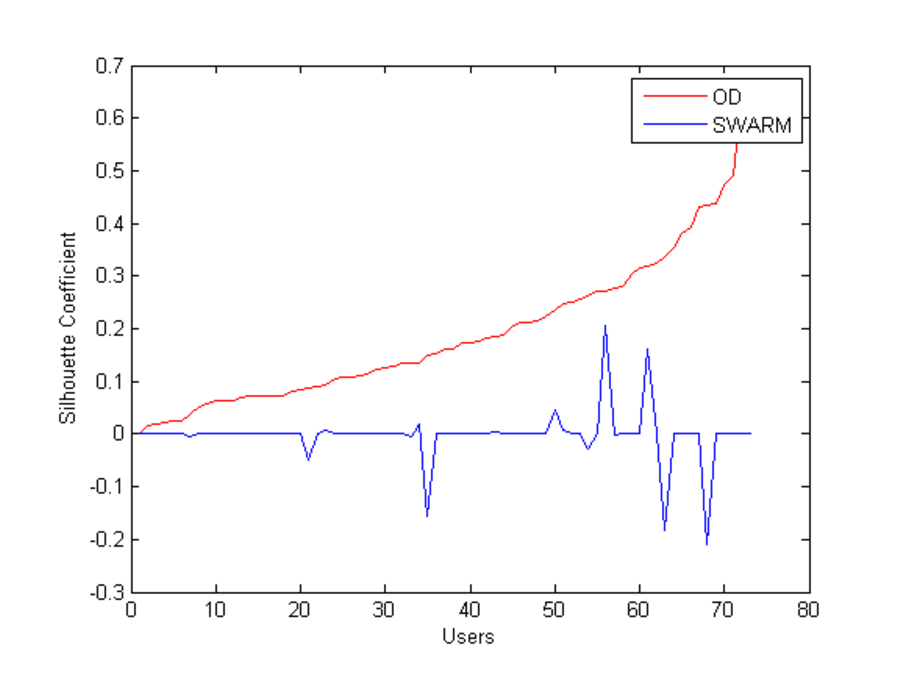
\includegraphics[scale=0.6]{figs/swarm_od_silcomparison.eps}
\caption{Silhouette Values of the resulting clusters for SWARM and OD- We perform significantly better over all users}
\label{fig:SWARM_OD}  
    \end{subfigure}%
	\begin{subfigure}[t]{.5\textwidth}
        \centering
        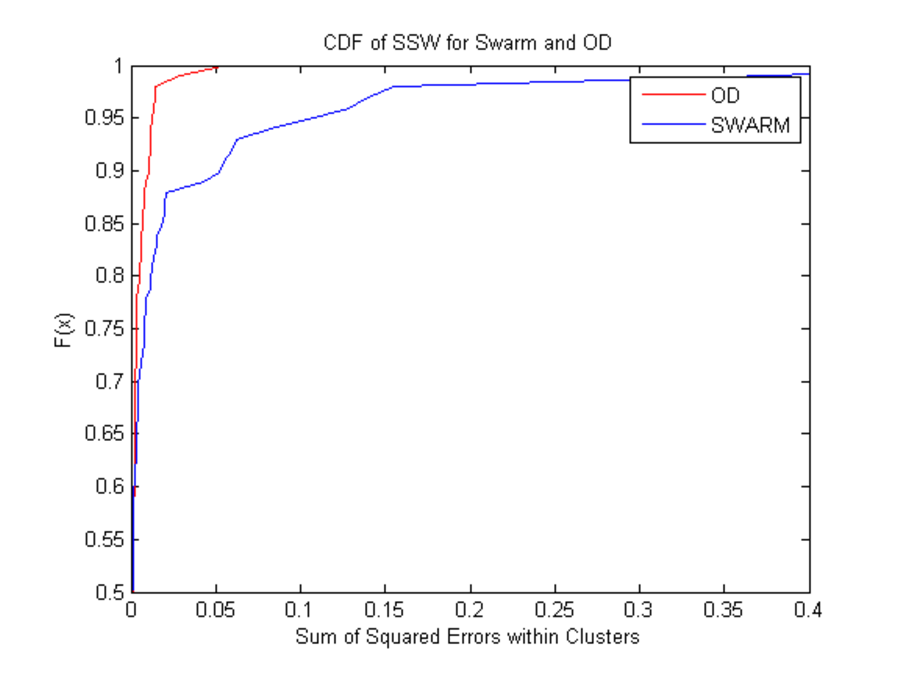
\includegraphics[scale=0.6]{figs/swarm_od_ssw.eps}
\caption{SSW Values of the resulting clusters for SWARM and OD- Our SSW error is lesser than SWARM over all users}
\label{fig:SSW_SWARM} 
    \end{subfigure}
    \caption{SWARM comparisons}
    \label{fig:swarm}       
\end{figure*}


\subsubsection{TraClus}
TraClus looks at the sub-trajectory level, and clusters trajectories on the basis of the similarities between those sub-trajectories. In the first phase, it partitions the trajectories into segments, and in the second phase, it clusters the partitions together using a DBSCAN-like technique.The problems with TrajClus are
\begin{itemize}

\item
The similarity measure between any two partitions is defined as a weighted sum of the perpendicular distance, parallel distance and the angular distance between the partitions. Here, three quantities with different units are being merged together, so when two partitions are similar, it is difficult to say which distance contributed to the similarity. Also, this creates a problem in arriving at the neighbourhood parameters. 

\item
 There are two parameters used in this algorithm, \textit{epsilon} and \textit{minLns}. \textit{epsilon} defines the neighourhood reach of each of the partition, and minLns is the minimum number of Partitions required in the neighbourhood for it to be considered as a cluster. The authors suggest a simulated annealing technique to arrive at the value of epsilon , and from that value, further calculate the value of minLns. But, because the algorithm is highly associative, nearly all the partitions end up in one cluster, thus not identifying the correct movement summaries. 
   
   
\begin{figure*}
    \centering
    \begin{subfigure}[t]{.5\textwidth}
        \centering
        \includegraphics[scale=0.4]{figs/TrajClus_full.jpg}
        \caption{All the trajectories of an example user }
\label{fig:TrajClus_full}  
    \end{subfigure}%
	\begin{subfigure}[t]{.5\textwidth}
        \centering
        \includegraphics[scale=0.4]{figs/TrajClus_cluster.jpg}
\caption{Cluster reported by TraClus}
\label{fig:TrajClus_cluster}  
    \end{subfigure}
    \caption{TraClus Final cluster reported}
    \label{fig:traclus}       
\end{figure*}


\item

TrajClus does not give enough weightage to the direction of the line segment. In cases like animal movement or hurricane movement, this makes sense, because there wont be many cases of trajectories in different directions in a flock or cluster. But when it comes to human movement pattern, directions play a very important role in determining the movement summaries of a person. TrajClus overlooks it and clusters two trajectories in different directions in the same cluster.

\begin{figure}
\centering     
\includegraphics[scale=0.3]{figs/direction.jpg}
\caption{Trajectories with different directions clustered together by TrajClus}
\label{fig:TrajClus_direction}  
\end{figure}

\end{itemize}
\subsubsection{Next Location Prediction}
Another way to test the summarization of the movement patterns is to test a query trajectory and plot its predicted next location/destination as predicted by all the methods.

The next location prediction is done by the following algorithm:
\paragraph{Explanation of the algo}
For any query trajectory, resample, and compute similarity with the median trajectories of all summary clusters. Report the one with the maximum similarity. 


Let $g(i)$ be the probability of the summary $i$. Given an input traj $t_{\operatorname{in}}$, compute the distance (in meters or so) $d(i,t_{\operatorname{in}})$ between summary $i$ and $t_{\operatorname{in}}$. Now the probability that this sub-trajectory lies within summary $i$ is given by
\begin{eqnarray}
p(i,t_{\operatorname{in}}) = \frac{1}{\sqrt{2 \pi} \sigma_{t}} \mathrm{e}^{-0.5 \left( \frac{d(i,t_{\operatorname{in}})}{\sigma_{t}} \right)}
\end{eqnarray}
Here we assume that the input trajectory is a noisy input from GPS samples. $\sigma_{t}$ is the standard deviation of the sub-trajectory distance. For now take, $\sigma_{t} = \sigma_{p}$, where $\sigma_{p}$ is the standard deviation of the GPS sampling a location (value is 15.61, which is the 95-th percentile of GPS considering 30 m error). It should ideally be standard deviation introduced when we compute distance between 100 points of a path

For each of the methods compared, we plot the CDF of the error of the predicted destination for the Top-3 Closest clusters to each of the query trajectories. Each of the graphs contain 4 plots, each one varying the number of sample points given to the query trajectory. We have plotted the errors for query trajectories with 10\%, 25 \%, 50\% and 90\% of the sample points. 

\begin{figure*}
    \centering
    \begin{subfigure}[t]{.5\textwidth}
        \centering
        \includegraphics[scale=0.4]{figs/dtw_top.jpg}
        \caption{CDF of error in predicted destination for 1st closest cluster using DTW}
    \end{subfigure}%
	\begin{subfigure}[t]{.5\textwidth}
        \centering
        \includegraphics[scale=0.4]{figs/dtw_top2.jpg}
        \caption{CDF of error in predicted destination for 2nd closest cluster using DTW}
    \end{subfigure}
    \begin{subfigure}[t]{.5\textwidth}
        \centering
        \includegraphics[scale=0.4]{figs/dtw_top3.jpg}
        \caption{CDF of error in predicted destination for 3rd closest cluster using DTW}
    \end{subfigure}
    \caption{CDF of the error in predicted destinations for the top 1,2,3 closest clusters for \emph{DTW}}
    \label{fig:nextloc_DTW}       
\end{figure*}

\begin{figure*}
    \centering
    \begin{subfigure}[t]{.5\textwidth}
        \centering
        \includegraphics[scale=0.4]{figs/od_top.jpg}
        \caption{CDF of error in predicted destination for 1st closest cluster using OD}
    \end{subfigure}%
	\begin{subfigure}[t]{.5\textwidth}
        \centering
        \includegraphics[scale=0.4]{figs/od_top2.jpg}
        \caption{CDF of error in predicted destination for 2nd closest cluster using OD}
    \end{subfigure}
    \begin{subfigure}[t]{.5\textwidth}
        \centering
        \includegraphics[scale=0.4]{figs/od_top3.jpg}
        \caption{CDF of error in predicted destination for 3rd closest cluster using OD}
    \end{subfigure}
    \caption{CDF of the error in predicted destinations for the top 1,2,3 closest clusters for \emph{OD}}
    \label{fig:nextloc_OD}       
\end{figure*}

\begin{figure*}
    \centering
    \begin{subfigure}[t]{.5\textwidth}
        \centering
        \includegraphics[scale=0.4]{figs/lp_top.jpg}
        \caption{CDF of error in predicted destination for 1st closest cluster using LP}
    \end{subfigure}%
	\begin{subfigure}[t]{.5\textwidth}
        \centering
        \includegraphics[scale=0.4]{figs/lp_top2.jpg}
        \caption{CDF of error in predicted destination for 2nd closest cluster using LP}
    \end{subfigure}
   \caption{CDF of the error in predicted destinations for the top 1,2 closest clusters for \emph{LP}}
    \label{fig:nextloc_LP}       
\end{figure*}

\begin{figure*}
    \centering
    \begin{subfigure}[t]{.5\textwidth}
        \centering
        \includegraphics[scale=0.4]{figs/swarm_top.jpg}
        \caption{CDF of error in predicted destination for 1st closest cluster using SWARM}
    \end{subfigure}%
	\begin{subfigure}[t]{.5\textwidth}
        \centering
        \includegraphics[scale=0.4]{figs/swarm_top2.jpg}
        \caption{CDF of error in predicted destination for 2nd closest cluster using SWARM}
    \end{subfigure}
   \caption{CDF of the error in predicted destinations for the top 1,2 closest clusters for \emph{SWARM}}
    \label{fig:nextloc_SWARM}       
\end{figure*}


Some of the observations from the next location prediction results are as follows:\\
Our Approach and LP predict the destination of \emph{82\%} of the trajectories with less than 10km error for closest cluster. 
DTW also is very close with prediction \emph{80\%} of the trajectories, but SWARM fares very badly with just \emph{5\%} of the trajectories' destination predicted. SWARM cannot detect the third closest cluster for any of the input trajectories. 



%Extra Graphs --->
%\begin{figure}
%\centering     
%\includegraphics[scale=0.3]{figs/testing_sil.jpg}
%\caption{Comparison of silhouette coefficients for different schemes: OD- and LP-based clustering outperform existing mechanism. }
%\label{fig:sil_cdf}  
%\end{figure}
%
%The CDF plot shows that  DTW is very similar to our approach in terms of clustering effectiveness, but SWARM does a very poor job. 
%
%\subsubsection{Average Trajectories Per Cluster}
%Number of clusters with large number of trajectories in it is better (Figure~\ref{fig:avg_cdf} and ~\ref{fig:avgtop_cdf}). 
%
%\begin{figure}[H]
%\centering     
%\includegraphics[scale=0.3]{figs/avg.jpg}
%\caption{CDF of Average trajectories per cluster for LP-DTW-OD}
%\label{fig:avg_cdf}  
%\end{figure} 
%
%\begin{figure}[H]
%\centering     
%\includegraphics[scale=0.3]{figs/avgtop.jpg}
%\caption{CDF of Average trajectories per top-k clusters for LP-DTW-OD}
%\label{fig:avgtop_cdf}  
%\end{figure} 
%
%\subsection{Computation Time}
%
%\begin{figure}[H]
%\centering     
%\includegraphics[scale=0.3]{figs/time_log.jpg}
%\caption{Computation time  for LP-DTW-OD}
%\label{fig:time_cdf}  
%\end{figure} 
%
%
%



%\subsubsection{Visualization at various granularity }
%%\rednote {Remove later if needed}
%
%\begin{figure*}
%\centering   
%\includegraphics[scale=0.6]{figs/demo.jpg}
%\caption{Visualization at various zoom levels}
%\label{fig:demo}  
%\end{figure*}
%
%\subsubsection{Case Study: Reported Final Clusters from each method}
%
%We take up a sample case, and show the snapshots of the final clusters as reported by all the different methods. DTW and OD have similar final clusters whereas SWARM reports only final clusters. 
%
%
%\begin{figure}
%\centering     
%\includegraphics[scale=0.4]{figs/snapshot_swarm.jpg}
%\caption{Snapshot of clusters reported by SWARM }
%\label{fig:casestudy_swarm}  
%\end{figure} 
%
% 
%\begin{figure}
%\centering     
%\includegraphics[scale=0.4]{figs/snapshot_od.jpg}
%\caption{Snapshot of clusters reported by OD}
%\label{fig:casestudy_od}  
%\end{figure} 
%
%\begin{figure}
%\centering     
%\includegraphics[scale=0.4]{figs/snapshot_dtw.jpg}
%\caption{Snapshot of clusters reported by DTW}
%\label{fig:casestudy_dtw}  
%\end{figure} 
%
%\iffalse
%The table below shows the statistics of the top k clusters and the number of trajectories 
%
%\begin{table*}
%	\centering
%		\begin{tabular}{|c|c|c|c|c|} 
%			\hline
%			Method&DTW&SWARM&TrajClus&OD\\
%			\hline
%			Number of Clusters Reported&1&4&0&18\\
%			Number of trajectories in top 3 Clusters & 5&36,15,13&0&38,37,29\\
%			\hline
%		\end{tabular}
%	\caption{Comparison for case study}
%	\label{tab:case_study}
%\end{table*}
%\fi


\section{Related Work}
Trajectory similarity and trajectory clustering has been studied widely over the past few years due to the growing availability of data to experiment with. There have been various papers proposing new similarity measures and many others which propose an end to end framework for clustering trajectories. More than individual movement summary, people have mainly considered hurricane data, and animal movement pattern. The problem of of finding individual moment summary has not yet been addressed by anyone to the best of our knowledge. We divide the literature review into various section and discuss the papers published in each of the sections respectively.
\subsection{Trajectory Similarity}
The most commonly used similarity measure for any kind of time series similarity is the LP- norm similarity. In \cite{lp1}, the authors talk about using Euclidean distance to measure similarity, coupled with Discrete fourier transform to reduce the dimensionality and R-tree was used for indexing. Various Fast and efficient methods for indexing and retrieval of similar series , when the similarity is defined by the Euclidean similarity are proposed in \cite{lp1},\cite{lp2},\cite{lp3},\cite{lp4},\cite{lp5} . 
The main problem with Euclidean distane is its inability to handle noise and local time shifting. In order to overcome this, exploration in other techniques began. Berndt \emph{et al.} \cite{dtw} introduced Dynamic Time warping which allowed  a time series to be stretched so as to match the query series. In variations to DTW, Vlachos \emph{et al.} \cite{Vlachos2002} applied Longest Ccommon Subsequence(LCSS) measure, and Chen \emph{et al.}\cite{Chen2005} applied  Edit Distances on Real Sequences(EDR). But all these measures, i.e., DTW, LCSS , and EDR are not metrics and don not follow triangle inequality. As an improvement, Chen \emph{et al.}\cite{Chen2005} introduced Edit Distance with Real Penalty (ERP) which handled local time shifting and is a metric. In \cite{simcomp}, Wang \emph{et al.} compare six widely used similarity measures including measures such as Euclidean distance, DTW, ERP, EDR and LCSS and their performances as trajectory similarity measures. They use a taxi dataset to evaluate and compare the results. Sankararaman \emph{et al.} \cite{simcomp2} have presented an extensive experimental study comparing the various similarities and also proposing a similarity of their own for trajectories. 

\subsection{Trajectory Clustering}
In \cite{gaffney1999trajectory}, Gaffney \emph{et al.} talk about trajectory clustering using the Expectation Maximization algorithm. Nanni \emph{et al.} \cite{nanni2006time} came up with an adaptation of a density-based clustering algorithm for trajectories.Zhang \emph{at al.} came up with a kernel density estimation based approach for the clustering of spatio-temporal trajectories in \cite{Zhang}.In \cite{su2015making}, the authors propose a system to generate text summaries of the trips made by people using a partition and summarization approach. [\cite{mapmatch1},\cite{mapmatch2},\cite{mapmatch3}] talk about trajectory clustering after snapping the trajectories on some base map. Map matching constraints the trajectories to a specific network, and various other avenues open up in terms of defining similarity.

\subsection{Subtrajectory Clustering}
Li \emph{et al.}\cite{Li2010} talk about moving clusters and detecting closed swarms for trajectories. Moving clusters in trajectory clustering is talked about in \cite{flock1},\cite{flock2},\cite{flock3} as well. Lee \emph{et al.} \cite{Lee2007} propose a partition and grouping framework for clustering trajectories. They try to cluster trajectories which have a common course for most of the path, or some sub trajectory similarity is high, but then start to diverge. Lee \emph{et al.} talk about a classification algorithm for trajectories based on two methods - hierarchical region based and trajectory clustering based classification. 

\subsection{Trajectory Preprocessing and Representative Trajectory}
Li \emph{at al.} and Zheng \emph{et al.} have a proposed a heuristic to cut meaningful trajectories from a stream of $<latitude, longitude, timestamp>$ three tuples in \cite{trajcut1,trajcut2} respectively. In \cite{trajcut3}, Zheng gives a complete overview on trajectory data mining which also contains a section on trajectory data pre-processing.  
Buchin \emph{et al.} talk about various ways to find the representative or median trajectories for a group or cluster of trajectories in \cite{median1}.


\section{Conclusion}
\label{sec:conc}
We proposed a Hadoop-based \trajSummary system that inputs location traces and computes mobility summary for individual users. The mobility summary is computed by using clustering algorithms on trajectories. We discuss and evaluate the effectiveness of popular distance metrics and clustering algorithms for our application of creating user summaries. We show that $\UN$ metric provides a good abstraction for distance metric between trajectories for the usecase of creating user summaries. We propose three cluster identification techniques that are appropriate for \trajSummary. \thresh and \lthAware are parametric methods to identify optimal clusters. \modal is a non-parametric method that performs the best for creating effective user summaries. We evaluate our algorithms with Geolife data-set, and show that our algorithms outperform existing clustering mechanisms. 

In future, we want to develop this work for considering spatio-temporal clustering of user trips. We also would want to extend the work to other forms of location traces such as Call Detail Records. The challenge with such location traces is to develop techniques that can handle high-errors in space and infrequent sampling.

%% ADd the below at right places
%\section{Motivation}

\subsection{Trajectory Similarity}

\paragraph{Motivation  behind giving weight age to OD }

\par  The intuition behind the similarity measure is that whenever humans move, there is an intent behind the trip. Thus, the origin and destination have an important role to play. If someone is making a trip, the destination has to be of some importance to the person, and the origin should also mean something to him. Following this intuition, we have given more weightage to the points closer to the origin and destination. Another reason behind doing this is that we want to overlook tiny diversions in the route taken from a set pair of origin-destination. For example, for a user, if the trips he make from the office to his home are considered as one summary, and on some day if he takes a tiny diversion in the form of a by-lane rather than the main road, it should still be considered  in the same trip summary. Thus, the points closer to the origin and destination are given more importance than those in the middle. 

\paragraph{ Problems with existing metrics}

\par There are various existing metrics for computing similarity between trajectories like  Dynamic Time Warping(DTW), Edit Distance on Real Sequences (EDR), Longest Common Sub-sequence(LCSS), etc.  But the major problem with most of them is that they are not mathematical metrics and thus, do not follow triangle inequality. This might lead to inconsistent results in various situations, and mainly affect the clustering results. 
\paragraph{Problems with defining similarity when both spatial and temporal domain come into the picture}

\par Moving into the the domain of defining a spatio-temporal similarity between two trajectories brings in various questions of ambiguity. Are simiarlities between two trajectories which go on the same path 10 mins part same as that of two trajectories which go 1 km apart at the same time? Hence, a hierarchical approach for solving this problem is suggested so as to decouple the spatial and temporal similarities. We first come up with the trip summaries by looking only at the spatial values, and then in the next stage , bring in the temporal (time of the day aspect) aspect to gain further insights.

\paragraph{Denoising over using similarity measures resilient to noise}
\par For human trip movement, denoising can be done prior to trajectory processing, instead of making the similarity measures resilient to noise. Such similarity measures are computationally expensive, and do not yield accurate results in all cases.

\subsection{Trajectory Clustering}

Why hierarchical: We really dont know the number of clusters. We need to iterate over each k and then find out the optimal k. The time complexity of running k-means for 100's of ks and then finding out the optimal k is much more expensive than doing 1-shot hierarchical clustering and finding a good point to cut. %\rednote{Show the time graph for running k-means vs hierarchical}\rednote{Show complexity}

\subsection{Trajectory Summarization}

\par { Use cases for trajectory summarization}

Computing the trajectory or trip summaries of a person can answer various queries about the person. Some of them include 
	  \begin{itemize}
			\item Customer Profile: Give summary of a person's trips in a region -- both in space or time
			\item Next-Location Profile: What are the most probable trajectories to find a person between time x to time y (optional: given that the person is at location L at time t)
			\item Alerts: Alert when a customer is moving in an anomalous way
		\end{itemize}
Trip summaries can also be used for
		\begin{itemize}
			\item Insurance Usecase: Give summary of a person's trips that have good or bad speed profiles -- immaterial of the space or time
		\end{itemize}


\subsection{ Storing the summaries of a person}

\par We also propose a method of storing the trip summaries of  a person in a hierarchical fashion. By doing this, we can get an idea about how the person moves at various levels of granularity. We can also set the number of clusters to a particular value, and query his movement pattern for the top k prominent trips. This kind of storage also supports zooming into a particular summary and breaking it down further for other analytics.


\balance
\bibliographystyle{abbrv}
\bibliography{refs}
\end{document}